\documentclass{report}\usepackage[]{graphicx}\usepackage[]{color}
%% maxwidth is the original width if it is less than linewidth
%% otherwise use linewidth (to make sure the graphics do not exceed the margin)
\makeatletter
\def\maxwidth{ %
  \ifdim\Gin@nat@width>\linewidth
    \linewidth
  \else
    \Gin@nat@width
  \fi
}
\makeatother

\usepackage{Sweavel}

  
\lstset{breaklines=true} 	
\usepackage{geometry}                		
\geometry{letterpaper}                   		
\usepackage{graphicx}												
\usepackage{amssymb}
\usepackage{amsmath}
\usepackage[utf8]{inputenc}
\lstset{language=R}
\usepackage{listings}
\usepackage{float}
\usepackage{subcaption}

\usepackage{tikz}
\usetikzlibrary{shapes,arrows,chains}




\title{Comprehensive Exam Notes}
\author{Patrick Dylan Barry}
						

\begin{document}
\maketitle
\abstract{}
During my Ph.D. at the University of Alaska Fairbanks I needed to study for comprehensive exams.
My committee made up of Anthony Gharrett, Megan McPhee, David Tallmon, and Eric Anderson 
were tasked with choosing topics that I needed to master in order to graduate and continue on the 
Ph.D. track. During my first committee meeting they made a list of topics: Relationship/Parentage analysis,
population genetic theory, coalescence, inference models for molecular ecology, population conservation 
genetics as applied to fisheries management, evolutionary ecology of Pacific salmon, and molecular genetic 
methodologies and applications. This list scared the bejezus out of me, and so I decided 
 that a good way of studying for these exams would be to create a short book that 
might aid in my preparation and be a good resource for the future. I think this should be worthwhile even
if nothing more grows out of this than a study guide for my exams or possibly lecture notes for a course I 
instruct. A major consequence of this is that many of the examples that I will use come from salmon. Similarly,
many of the first few sections come from lecture notes that I took while in Tony Gharrett's Introduction to Genetics Course. 

\newpage

\tableofcontents

\newpage

\chapter{A Brief History of the field of Genetics}
Hooke (1665) coins the term 'cell' after observing cellular structure in cork.

Anton van Leeuwenhoek (1670s) invents compound-like microscope - observes animalcules.

Schwann (1847) - proposes animals made of tissues which were constructed of 'cells'
Matthias Jakob Schleiden - plant cell structure - cells appear to be building blocks for complex organisms

Spontaneous generation
Redi - flies prevented from laying eggs = no maggots
Spallanzani - boiling hay infusion no animalcules
Pasteur and Tyndall - put it to rest
 
 Pangenesis -
 Aristotle eggs and sperm interact in mysterious way
 Hertwig used sea urchins to show developing embryo
 Strssburger did the same in plants - nucleus was important. 
 
 Fixity of Species - Linnaeus 
 
 Chromossomes - late 1800's 
 Boveri
 Henkens
 Montgomery
 
 Correns and deVries discover Mendels work. 

\chapter{DNA - a review}
In this section I will briefly review the discovery of DNA and review basic principles that will facilitate the 
understanding of preceding chapters. 

\section{DNA as the hereditary material}
Major experiments that lead to the discovery of DNA as the hereditary material. 
Biological molecule mediates inheritance. 

Possibilites - Carbohydrate/polysaccharide,lipid, protein, nucleic acid
Griffiths 1928
Dawson 1931
Alloway 1933
Avery, McCarty \& MacLeod 1944
Hershey\&Chase 1952
Fraenkel-Conrat and Singer 1957
Chargaff 1950
Linus Pauling
Watson/Crick/Franklin
\section{DNA structure}
Nucleotides - Nucleosides etc. 
\section{Transcription}
Brief description of DNA to mRNA
\section{Translation}
Brief description of mRNA to protein

\section{Mitochondrial DNA (mtDNA)}
\subsection*{History and Description}
Mitochondrial DNA (mtDNA) is, as its name suggests, DNA that is found within the mitochondria.
The word mitochondrion, coined by Carl Benda in 1898,  comes from the Greek word \textit{mitos} 
meaning ``thread" and \textit{khondrion} meaning ` `little granule''. Mitochondria are organelles 
found in most eukaryotic cells (plants, animals, and 
fungi) that generate adenosine triphosphate (ATP) from the phosphorylation of ADP through
cellular respiration. Details about the citric acid cycle (Krebs cycle) and the electron transport 
% should I add that mtDNA was discovered by two teams of scientists?%
chain which take pyruvate (the product of glycolysis) to produce ATP are extensivly covered in most 
introductory biology text books and are ommitted here. 

Nuclear and mtDNA have different evolutionary histories. It is theorized that mtDNA was derived from
the circular genome of an endosymbiotic bacteria ~1.5 billion years ago. This theory was first 
described by Schimper who in 1883 noticed striking similarties between chloroplasts within green plants and 
freeliving cyanobacteria. The theory was later formalized by Mereschkowski, a Russian botanist, in 1910 and 
 further advanced by Lynn Margulis in 1967. 

Mitochonrial DNA in multicellular organisms is cirular and double stranded. In unicellular organisms mtDNA
is linearly organized DNA with telomeres and telemorase. In mammals, mtDNA encodes 37 genes (13 proteins, 
22 tRNAs, and the large and small subunits of the rRNA). The guanine rich strand, referred to
as the heavy strand (H-strand) encodes 28 genes, while the cytosine rich strand or light strand (L-strand)
endoceds the 9 other genes. In addition to these coding regions is the control region (CR) that is
responsible for initiating replication and transcription. The CR, sometimes refered to as the DLP,
is composed of the displacement loop (D-loop) and associated transcription promoter regions. 

\begin{figure}[h]
\centering
  \begin{subfigure}[b]{.5\linewidth}
    \centering
    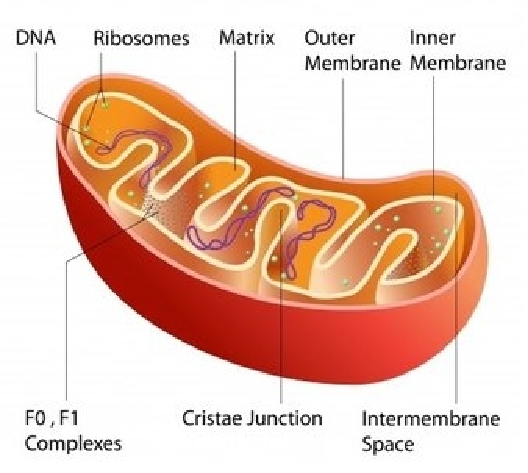
\includegraphics[width=.7\textwidth]{images/mito.pdf}
    \caption{}\label{fig:MGpro}
  \end{subfigure}%   
  \hfill
  \begin{subfigure}[b]{.5\linewidth}
    \centering
    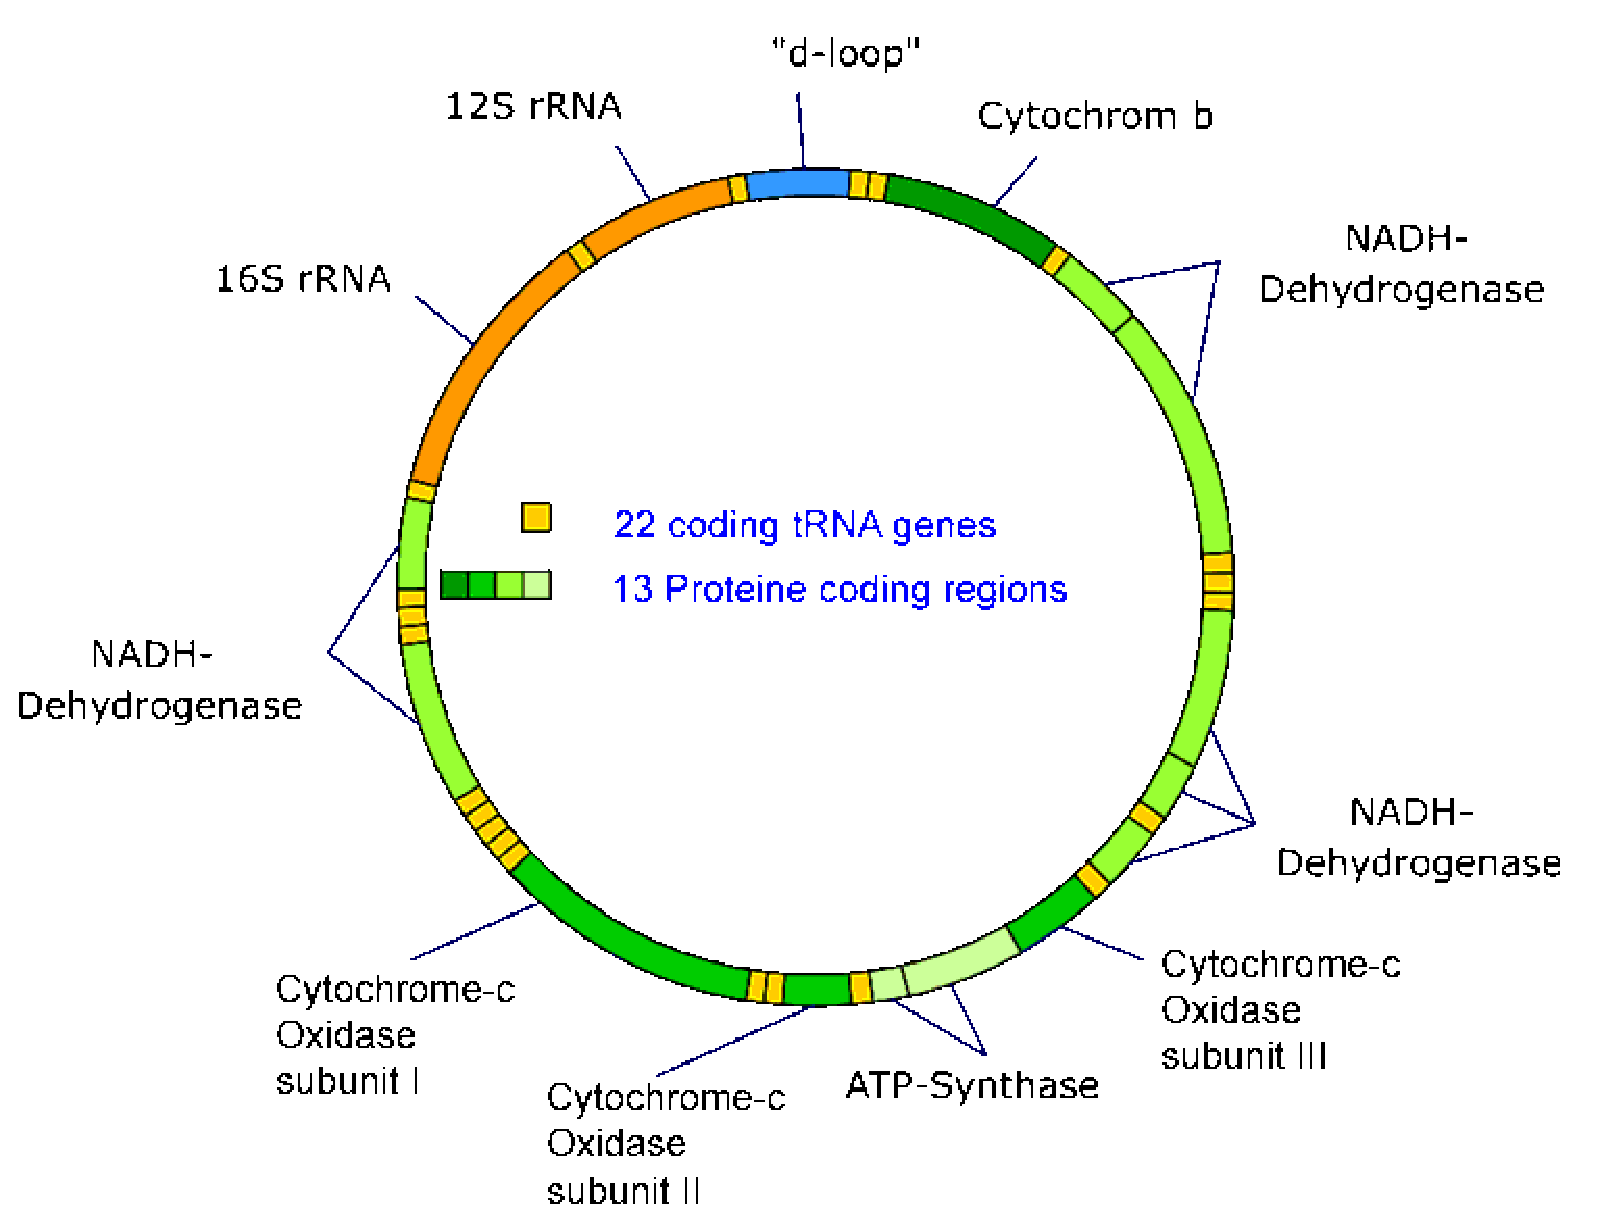
\includegraphics[width=.99\textwidth]{images/mtDNA.pdf}
    \caption{}\label{fig:MGchem}
  \end{subfigure}%    
  \caption{(a)   (b) }\label{fig:MG}
\end{figure}

There are a few characteristics that make mitochondria a particularly appealing marker to molecular ecologists, 
however recent research has started to question the assumption that these traits hold true
across a wide range of taxa (for detailed critiques see White et al. 2008 and Galtier et al. 2009). 

\subsection*{Inheritance}
First, mtDNA was thought to follow strict maternal inheritance in the 
majority of animals (Birky 1978 \& Dawid and Blackler 1972). Paternal DNA is eliminated at different steps of 
fertilization depending on the taxa. In crayfish, which lack flagellum on their sperm, mtDNA is abscent from
mature sperm Moses 1961 and thus cannot be inherited from the father. In the tunicate \textit{Ascidia nigra},
paternal mtDNA is blocked from entering the egg preventing paternal 
inheritance( Ursprung and Schabtach 1965). In both cow and monkeys
Sutovsky et al. (1999) suggest that ubiquination of mitochondria that occurs during spermatogenesis tags
paternal mtDNA molecules for destruction by proteasomes and lysosomes in the embryo before the 
third embryonic cleavage. Although many studies have suggested otherwise and have been refuted (for
a good review see Galtier et al. 2009). 

Why is paternal DNA excluded from the cell? Bromaham 2003 proposes that 
(1) 


\subsection*{Evolution of mtDNA molecule}
The bacterial genome from which mtDNA arose has gradually shrunk over time. Genes from the 
original genome have been transfered either to the nucleus or to other organelles. As genes are 
transposed to the nucleus a copy can remain in the mitochondria making nuclear-mitocondrial dna 
(\textbf{numts}).  

Selection for small genome size. Selective size advantage of faster replication

Small variations in mtDNA length is generally a result of homopolymer tracts generated by replication 
slippage. Larger differences may be due to duplication or deletions -> might be due to slippage as well?

Aerobic respiration takes place within the mitochondria and a major byproduct of ATP synthesis are
reactive oxygen species, specifically superoxide and hydrogen peroxide. These free radicals produce a 
highly mutagenic envornment for mtDNA. This coupled with
a limited repair mechanism leads to a much higher mutation fixation rate. 
Bogenhagen 1999 indicates that mtDNA can conduct base-excision repair, but cannot
accomplish nucleotide excision repair, nor mismatch repair. Mutation rates vary among taxa.
A universal molecular clock cannot be assumed. There also exists quite a
bit of heterogeneity in mutaiton rate among mtDNA loci. The 12s and 16s rDNAs are more conserved
than the CR. This is due to functional constraints on the proteins encoded.
The CR for vertebrates is often divided into three parts based on base composition and mutational
model (Review Saunders \& Edwards Molecular Evolution 2000 51 97-109).  

Transitions are more common than tranversions


Gene content and order has remained conserved among vertebrates, but some rearrangements have
been observed. Comparisions of sea urchins and vertebrates show that tRNA genes are highly mobile with 
tanspositions and inversions occuring.  

Zhang and Hewitt 2003 ``mitochondrial DNA can be the cause of fortune, regret or headache'' in describing
the selection of mtDNA over other marker types. In plants the mutational rate is very slow Wolfe 1987, but 
it seems that mutational rates for plants is highly variable. Cho, Y 2004 show some of the highest mutational
rates in plants! Very high recombination rate Palmer and Herbon 1988.



for the most part homoplasmic -> single mtDNA sequence predominates all cells of tissues in the 
organism
new muation add to a hteroplasmic condition - 2 genotypes in 1 individual. Not really the case!
mutations accumulate rapidly in nucleotide positions that have less selective constraints - protein coding
then decrease Brown et al 1979. -> rapid evolving sequences are more useful for population level studies


\subsection*{mtDNA in molecular ecology}


Population geneticists have used mtDNA to asses two salient questions: (1) what is the 
state of the exisitng genetic variation in the population and (2) identify reproductivly isolated
populations. mtDNA displays substantial variation among individuals within and among 
populaitons. 1970s to 1990 restriction length polymorphism (RFLP)
analysis of mtDNA dominated phylogenetics. 'Raw data' was restriction fragment 
digestion profiles - or restriction maps.
The presence/absence of restriction sites could be used as qualitative data for parsimony trees. 

corrleation between mtDNA diversity and nuclear diversity?

Maternally inherited means it is a 
promising marker for population genetics. Recent events - colonization, introductions and population bottlenecks
sex biased dispersal
Assumes neutrality and negligible back-mutation. 


Mitocondrial psuedogens in the nuclear gemone complicate their use in population genetic studies. Lucily, 
back in the day geneticists used to isolate mtDNA from all nuclear DNA making this a moot point.  

The analysis of mtDNA has been a mainstay of phylogenetics since XXXX and is still being used 
mtDNA is a single molecule and as such represents loci that are completely linked. 
Despite differences in the mutational rate among loci, it is just one look 
at the evolutionary history. Stochastic processes such as drift as well as selection will influence all mitochondrion
loci. This look is also only the matrilineal history. Some studies have used both mtDNA
and noncombining regions of the Y chromosome to look at population structure differences 
among sexes. The effective
population size of mtDNA is at most (if we have 1:1 sex ratios) 1/4 that of nuclear autosomal DNA. A lower 
effective population size results in a faster lineage sorting rate and higher allele 
extinction rate. % rewrite this sentence to make it clearer!
Selection not a huge deal if character states (nucleotides) are still synapomorphic. Does effect estimation 
of divergence times though!


Two issues:
Incomplete lineage sorting can lead to discordanent gene and species trees constructued using mtDNA genotypes. 

If a female has all male offspring that mtDNA lineage ends after that generation. Let's assume that females produce daughters
according to a Poisson distribution with $\lambda = \mu$. The probability that a female will have no offspring in the next generation
is simply $exp^{-\mu}$ (see below). The loss after $G$ generations can be expressed as $P_G = e^{\mu(x-1)}$, where $x$ is the 
probability of loss in the previous generation. Avise et al. showed that the probability of survival of two or more mtDNA lineages
% read this paper and summarize here.

\begin{gather}
  P(\theta)=\frac{1}{\theta!}\lambda^\theta exp^{-\lambda}, \ E(\theta)=\lambda ,\; \&\,\; var(\theta)=\lambda \\
 P(0)=\frac{1}{0!}\mu^0 exp^{-\mu} \\
 P(0)= exp^{-\mu}
\end{gather}

\begin{Schunk}
\begin{Sinput}
# R code showing probability of losing an mtDNA lineage after 1 generation
off <- seq(from = 0, to = 10, by = 0.25)  # range of offpring you might have
d <- dpois(x = 0, lambda = off)  # calculate prob of 0 daughters for # offpring
plot(x = off, y = d, xlab = "Number of female offspring produced", ylab = "Probability of having only sons", 
    type = "l")
\end{Sinput}
\begin{Sinput}
# R code showing how many maternal lineages are lost depending on how many
# female offering on average are left (u)
gen <- seq(from = 1, to = 100, by = 1)
u <- c(0, 0.5, 1, 1.5, 2)
PSA <- matrix(data = NA, ncol = length(gen), nrow = length(u))
for (fo in 1:length(u)) {
    for (g in 1:length(gen)) {
        if (g == 1) {
            PSA[fo, g] <- exp(-u[fo])
        } else {
            PSA[fo, g] <- exp(u[fo] * (PSA[fo, g - 1] - 1))
        }  #else
    }  #loop over fo
}  #loop over g
plot(x = gen, y = PSA[1, ], xlab = "Generations", ylab = "Probability maternal mtDNA genotype is lost", 
    type = "l", ylim = c(0, 1))
for (p in 2:nrow(PSA)) {
    points(x = gen, y = PSA[p, ], type = "l", lty = p)
}
legend(x = "topright", inset = c(0.01, 0.1), bty = "n", legend = c(paste("u", 
    "=", u, sep = " ")), lty = seq(from = 1, to = nrow(PSA), by = 1), )
\end{Sinput}
\end{Schunk}


%Insert figure with both of the plots constructed above
\begin{figure}[htb]
\centering
  \begin{subfigure}[b]{.5\linewidth}
    \centering
    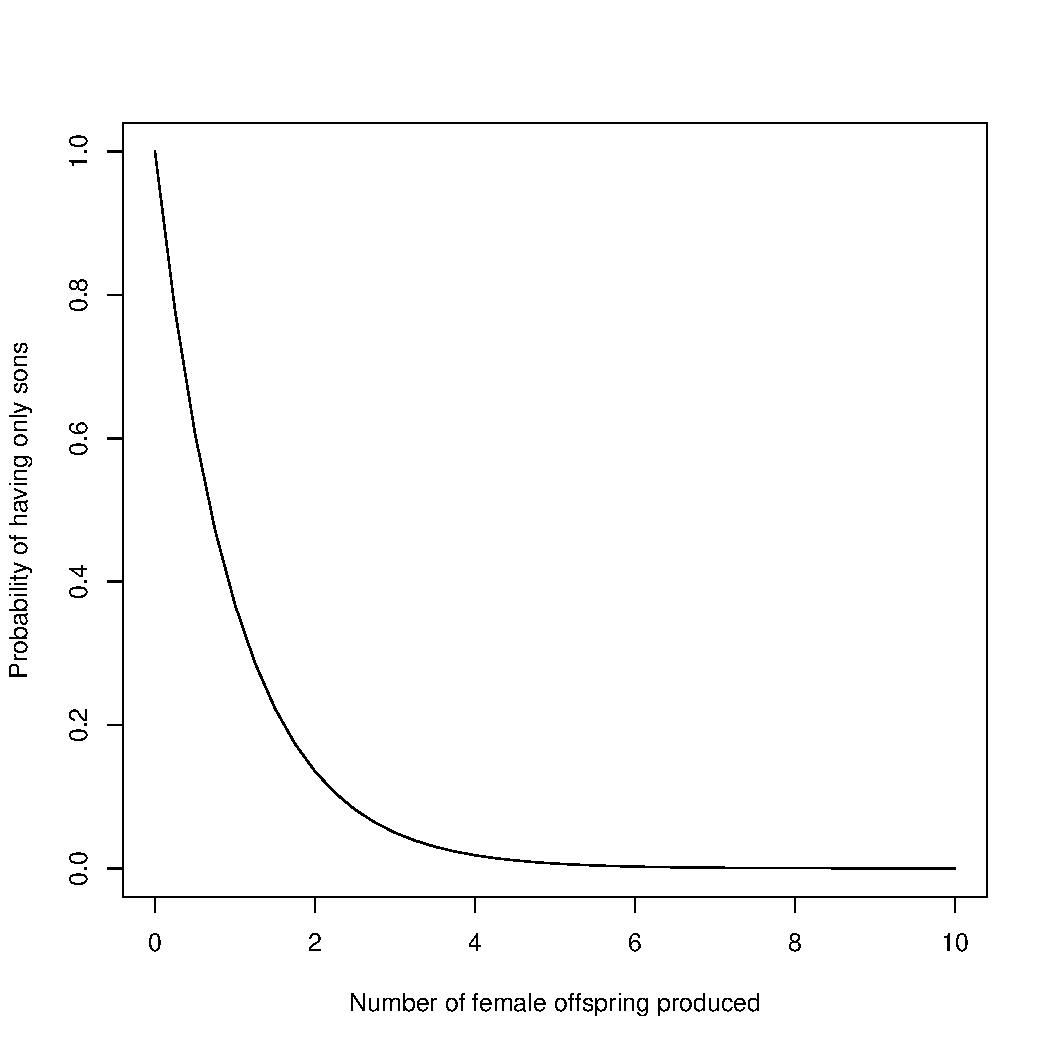
\includegraphics[width=.99\textwidth]{images/listings-unnamed-chunk-11.pdf}
    \caption{}\label{fig:chunk-11}
  \end{subfigure}%   
  \begin{subfigure}[b]{.5\linewidth}
    \centering
    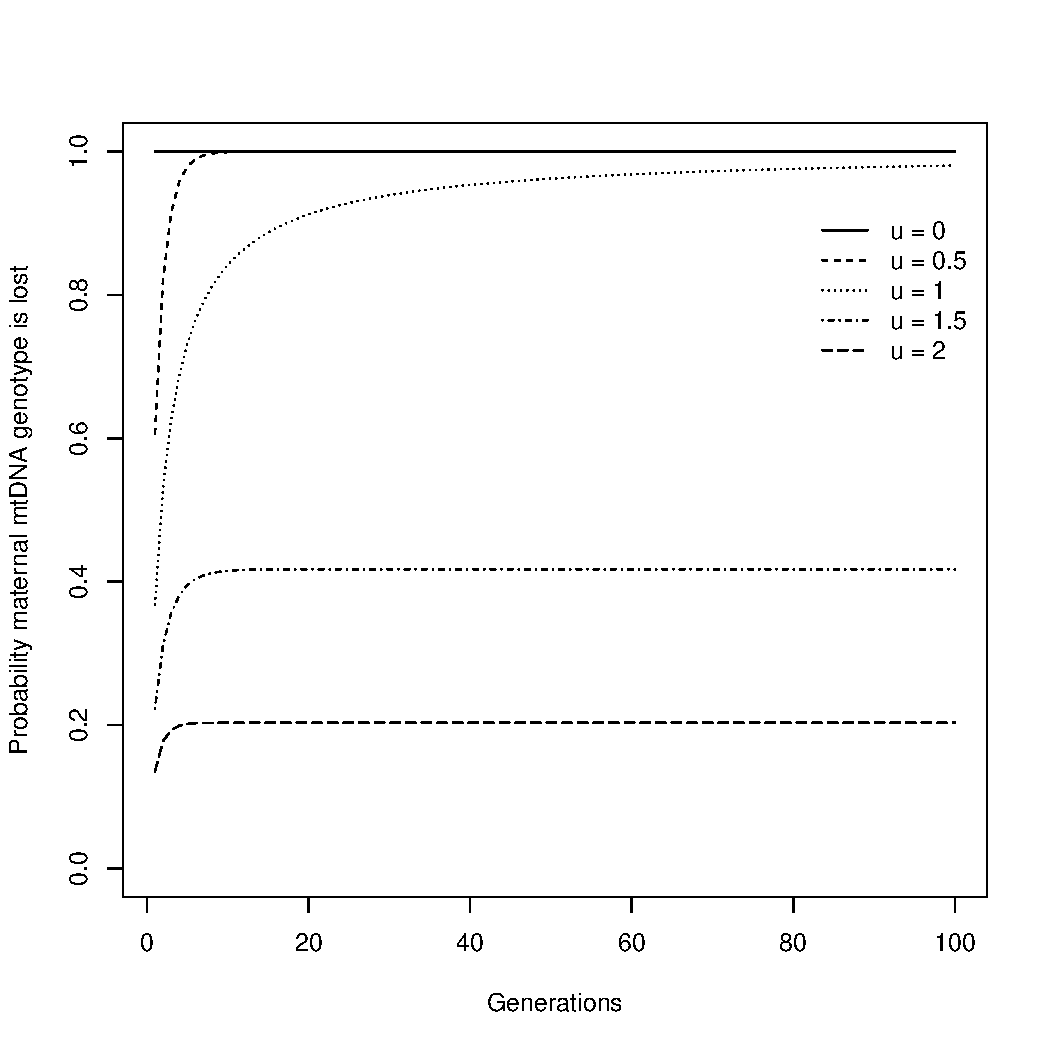
\includegraphics[width=.99\textwidth]{images/listings-unnamed-chunk-12.pdf}
    \caption{}\label{fig:chunk-12}
  \end{subfigure}%     
  \caption{(a) If we assume that females in a population produce female offspring according to
  the Poisson distribution with mean $\mu$, we can calculate the probability that a female mtDNA
  lineage is lost after one generation according to equation 3. It is fairly intuitive that the more female offspring
  produced, the higher then chance that a mtDNA haplotype lineage persists to the next generation. If on average
  only 1 female offspring is left, then there is a 37\% probability that the no daughters will
  be produced ending the mtDNA lineage for that family. We can also think of this in terms of how many maternal
  lineages will not persist. 
  (b) We can expand this and look at the persistence of mtDNA lineages through time. We can vary the average number
  of daughters produced by females ($\mu$). Again it is not surprising that if on average few daughters are produced, the
  time that it takes for an mtDNA lineage to go extinct is very short.}\label{fig:mtDNA_haplo_loss}
\end{figure}


Differential introgression
If two species existed we can imagine there being nuclear loci that are responsible for their reproductive isolation.
Patterns of introgression for nuetral nuclear loci will depend on how tightly linked they are to the markers 
responsible for isolation. mtDNA is unlinked to nuclear DNA and consequently the introgression of mtDNA variants 
will be much greater than for nuclear DNA. % good example of this from polar bears???
As a result inferences made from nuclear and mtDNA will be discordant. 



\subsection*{DNA Barcoding}
Recently, the use of short segments of mtDNA for taxonomic identification has been proposed. 
The basic theory is that we can use a short segment of DNA (a barcode) to identify an unidentified individual 
to species Hebert 2004. Later the amount of intraspecific divergence relative to 
interspecific divergence was proposed as a method
to identify cryptic species DeSalle, Egan \& Siddall, 2005. Many of these studies 
focused their efforts on the cytochrome oxidase I subunit (COI). This  approach 
requires extensive examination of the intraspecies divergence one would expect to see and then 
categorizing the interspecies divergence.


Due to incomplete lineage sorting the COI gene may not reflect the true relationships among species. 
This is one of the various critiques of using a single locus for species delineation 
(Moritz \& Cicero, 2004; Meyer \& Paulay, 2005; Will, Mishler \& Wheeler, 2005). 


\chapter{Molecular Genetic Markers}

\section{Phenotypic Data}

\section{Codominant Phenotypic Data}

\section{Allozymes \& Isozymes}
Lacking the ability to look directly at the entire genome, early genetic studies relied on small bits of translated 
genomic regions. DNA is transcribed to mRNA which is then translated to protein (See Chapter 2). Consequently,
proteins represent a way of looking at variation within DNA sequences. Proteins are polypeptides 
composed of strings of amino acids joined by covalent peptide bonds. Mutations within the protein coding 
regions can lead to different amino acids being incorporated into the polypeptide. Two general types of enzymes 
have been studied extensively:  isozymes and allozymes.  \textbf{isozymes} are all functionally similar forms of 
enzymes. \textbf{Allozymes} are a subgroup of isozymes that are coded by a single locus. 
Their name is derived from \textit{all}ele (alternative forms of a gene) and en\textit{zyme}. Data collection for 
both types of marker rely on enzymatic reactions and staining so isozymes and allozymes can often be 
investigated simultaneously.
Gel electrophoresis allows proteins to be separated based on their physical properties: charge, size, and shape. 
This method exploits the porous properties of a starch or cellulose acetate gel matrix and the differential charge 
of the amino acids that make up the allozyme. The rate of movement on a gel, \textit{u}, is dependent on the net
protein charge \textit{Q}, shape {r}, strength of the electric field \textit{d} and viscosity of the suspension 
medium \textit{n}:

\begin{equation*}
u=\frac{Qd}{4\pi^2n}
\end{equation*}

Charge differences among allozymes are resultant of the 
differential incorporation of positive (basic at neutral pH) amino acids lysine (Lys), arginine (Arg) and 
histadine (His) and negative (acidic at neutral pH) amino acids aspartic acid and glutamic acid. 

The strength of allozymes 


Cons: only observe non-synonous mutations, only look at water soluble proteins, 

\section{Restriction Length Polymorphisms (RFLPs)}

\section {AFLPs}


\section{Microsatellites \& Minisatellites}

\section{RAPiD}

\section{Sequencing}
Sequences are the ideal molecular data. If we had full genome sequences from all individuals in a study it would
be awesome. All other molecular markers discussed so far are just small snippets of the genome that we assume, if 
randomly sampled, are descriptive of the rest of the genome. Many of the previous 
markers rely on sequencing for their development. Sequencing has been around since the mid 1970's, but new
methods are currently being developed that improve upon these existing methods and make sequencing large
pieces of the genome a much more economical endeavor.

When comparing each type of sequencing method the pros and cons that would determine its utility and
eventually its use by researchers can be put into four broad categories:
\begin{itemize}
\item{\textit{Read length}} - Ideally we would be able to generate one long sequence, 
but usually reads are 100bp -1000bp and short fragments need to be aligned to make larger sequences.
\item{\textit{Speed}} - The time it takes to generate samples involves sample preparation, sequencing, scoring, and
alignment.
\item{\textit{Accuracy}} - One, if not the most important, attributes is generating good quality nucleotide scores. 
\item{\textit{Cost}} - If a method is not economical it is unlikely to be adopted by many research labs.
\end{itemize}
There are often tradeoffs between each of these attributes and what one lab values in generating sequence
data may not be what other labs value. As a result many labs differ in what technology they have adopted. The
platforms on which the technology is developed and implemented are not cheap and the technology is rapidly
changing. 



\subsection*{Sanger Method}
Sanger and Coulson developed the \textit{plus and minus} method in 1975. 
This method took used \textit{E. coli}
DNA pol I and bacteriophage T4 DNA pol with different nucleoside triposphates. 
DNA pol I first extends the primer copying the template strand in the presence of four 
deoxyriobotriphoshates, one of which is labeled with $^{32}P$.
This should create many copes of different length. From previous research it was 
shown that DNA polymerase in
the absence of one nucleotide, elongation would proceed until the 
position where the missing base should go. 
Using the partially elongated pieces from the first round of replication, Sanger \& Coulson 
used a \textit{minus} system, lacking one nucleotide, to deduce the sequences of each 
fragment up to the missing residue. Four different treatments
need to be done, one for each nucleotide. The \textit{plus} system is based on the 
research of Englund (1972) showing
that in the presence of a single nucleotide, DNA pol from T4 will 
degrade dsDNA from its 3' end. The exonuclease
activity is regulated by the presence of the nucleotides 
present - degradation only occurs in the absence of the 
nucleotides. This method was applied to the mixture obtained from 
the first elongation mixture produced, again
each nucleotide was done separately, so that when fractionated by 
electrophoresis bands will indicate the positions
of each residue in the sequence. The products in the \textit{plus} 
system will be one residue larger than those in 
the \textit{minus} system. 

\begin{figure}[h]
\centering
     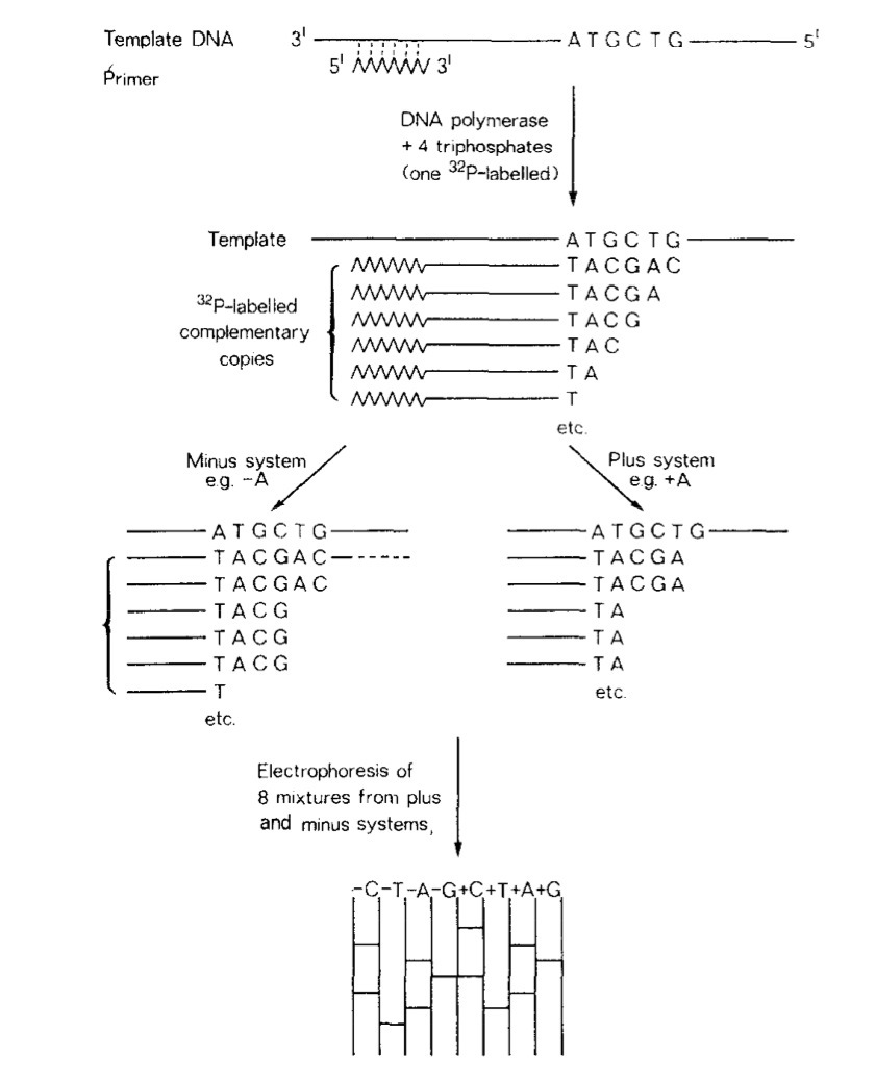
\includegraphics[width=.5\textwidth]{images/Plus_Minus.pdf}
    \caption{The \textit{plus minus} method of sequencing DNA developed 
by Sanger and Coulson in 1975}\label{fig:Plus_Minus}
\end{figure}

A couple problems were encountered. First, all possible length fragments should 
be created in the initial elongation
step. This was, often, not the case. Certain products were often found in high 
amounts while little or no yield of 
other fragment lengths were observed. Second, often artifact bands were 
observed making the inference of the
target sequence difficult. Third, the accuracy of the sequence was somewhat 
suspect and relied on cooberation
with amino acid sequence data. Fourth, it is only applicable to single stranded 
DNA. Lastly, 50 nucleotides in a couple days!  

In 1977 Sanger et al. proposed the method of DNA sequencing with chain-terminating
 inhibitors (\textbf{the Sanger
method}). Adkinson et al. 1969 observed that 2', 3'-dideoxythymidine triphosphate has
 inhibitory ability because ddT 
lacks a 3'-hydroxy group. If both ddTTP and dTTP are incubated in addition to the other three 
deoxyribonucleoside triphosphates with a primer and DNA polymerase 
fragments of different length 
will be produce each terminating 
where a dT should have been incorporated. The fragments can be fractionated by electrophoresis on an 
acrilamide gel. Mixtures with each terminator can be run side by side on an 
acrylamide gel to infer the complete 
sequence. 

\begin{figure}[h]
\centering
     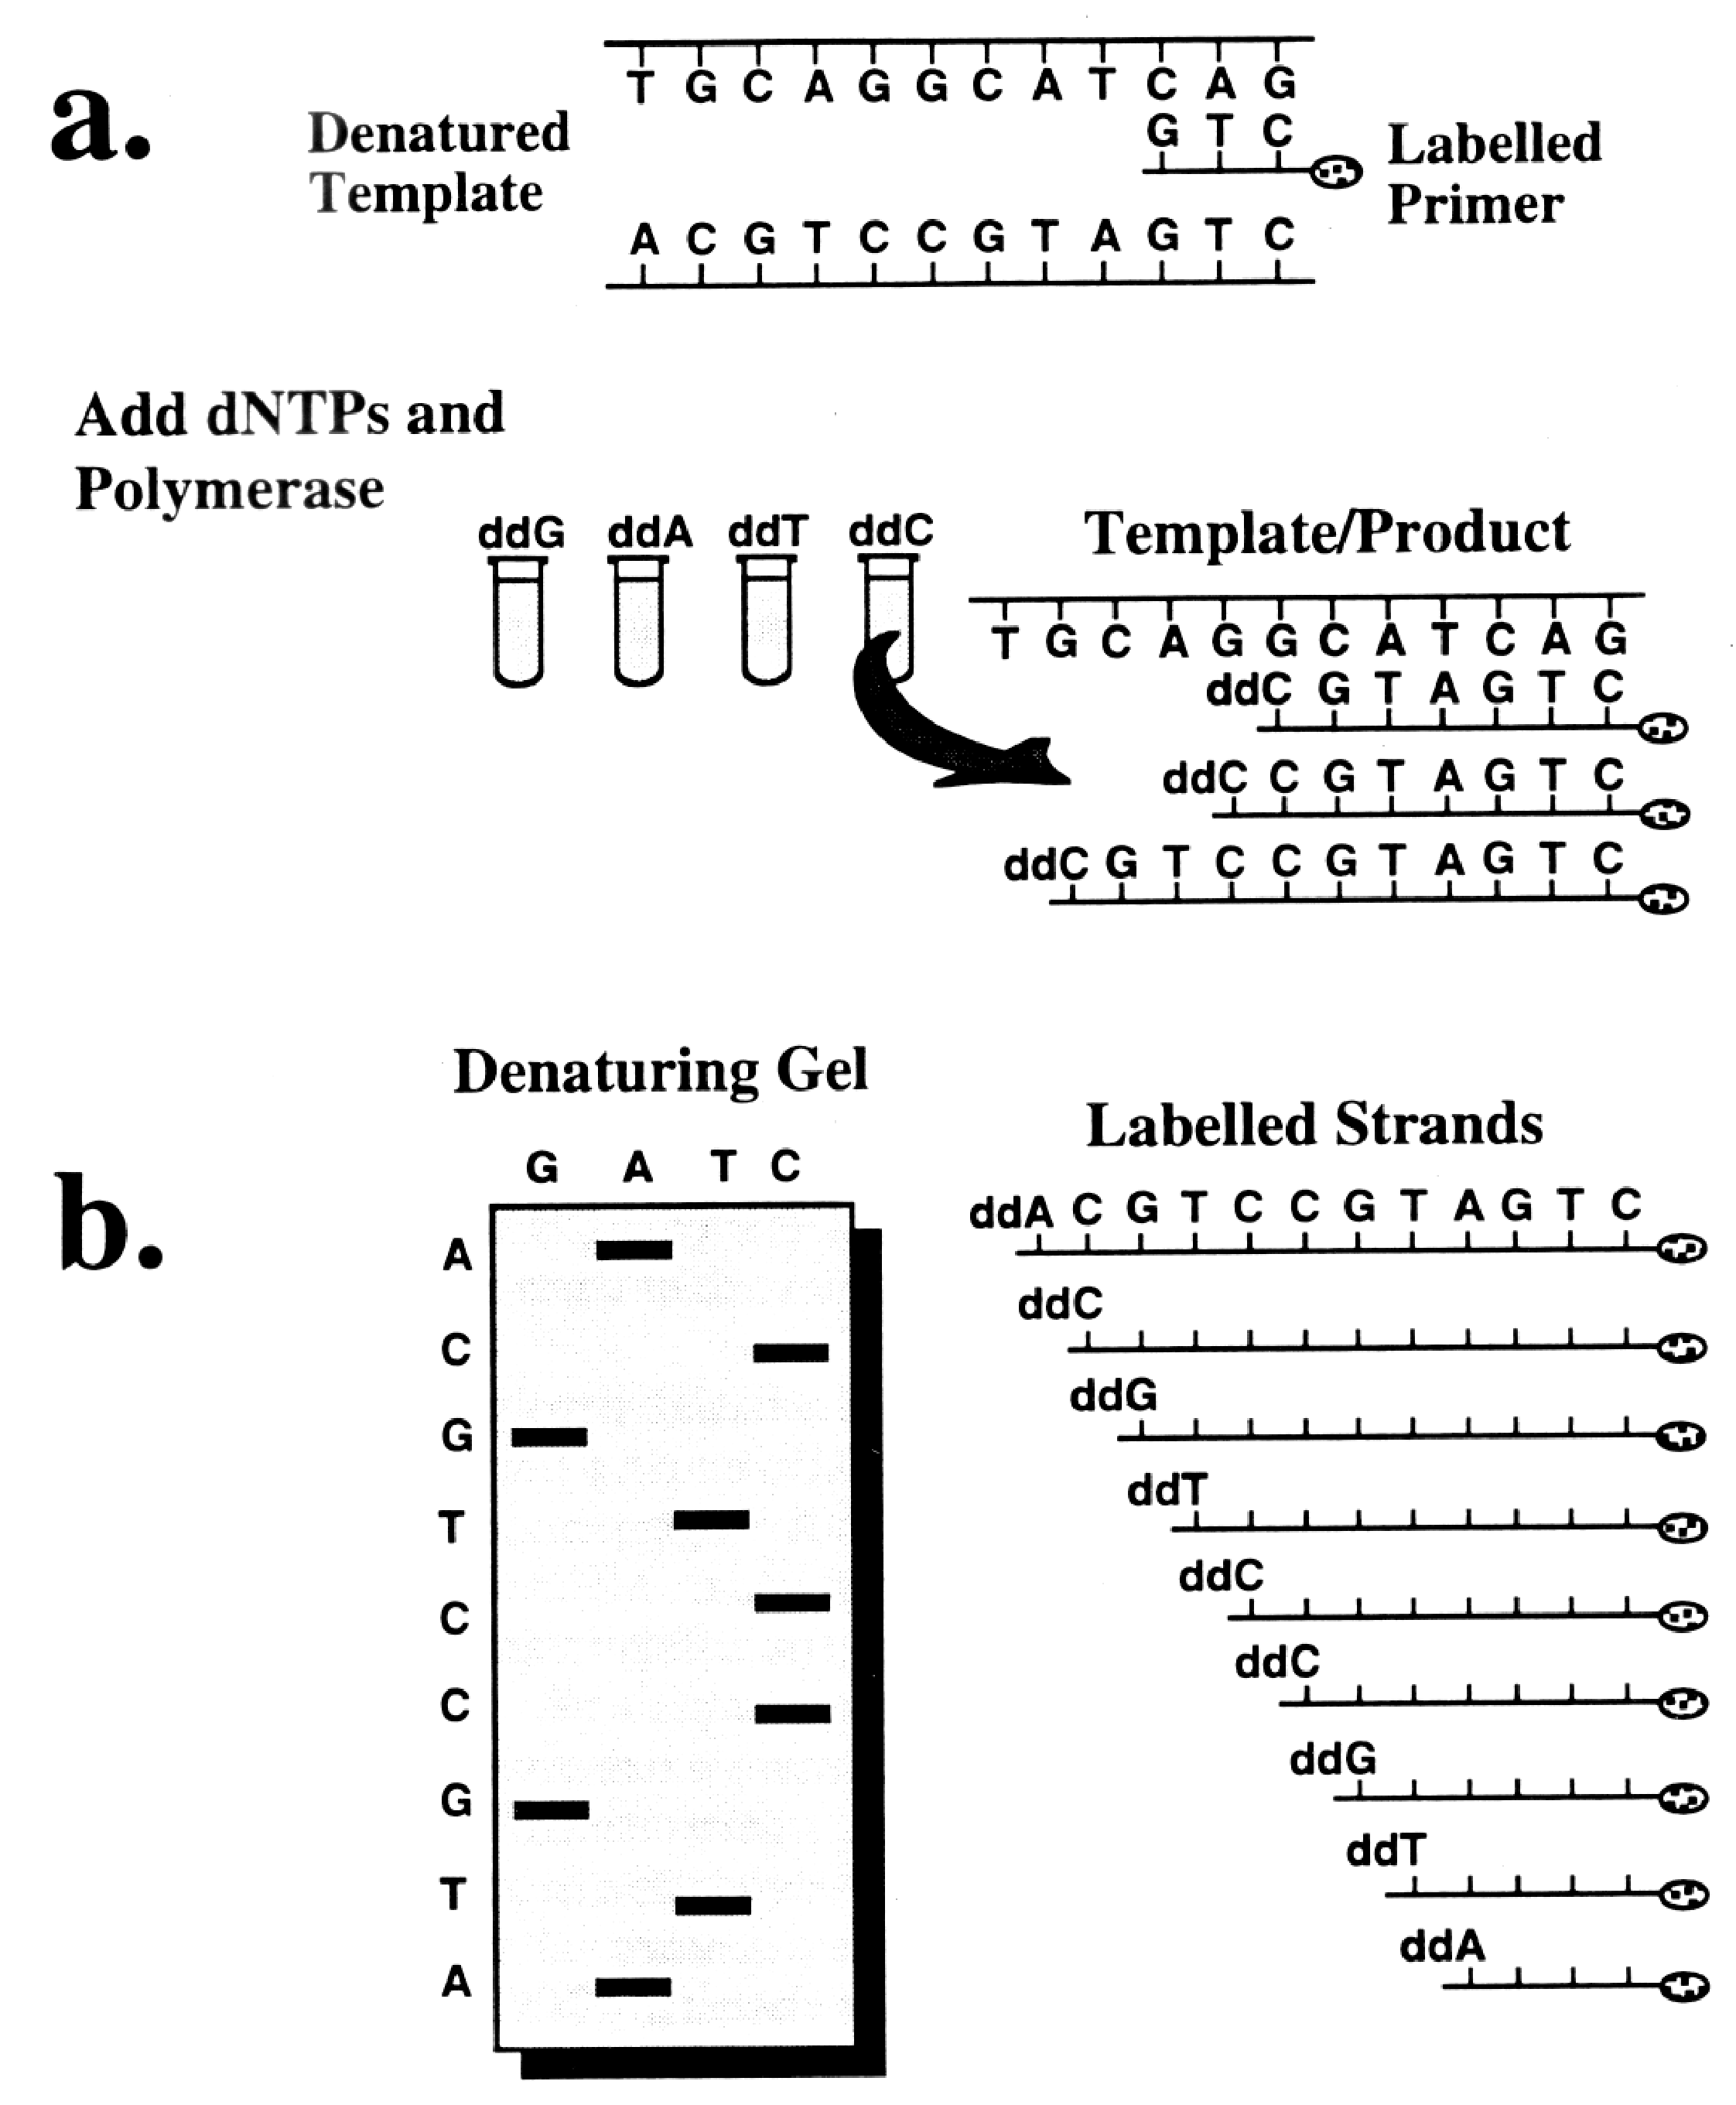
\includegraphics[width=.5\textwidth]{images/Sanger.pdf}
    \caption{The Sanger method of DNA sequencing by chain termination.}
\label{fig:Sanger}
\end{figure}


This method was better than the \textit{plus minus} method because it did not require a preliminary extension,
it only required one type of DNA polymerase, had fewer artifact bands, all individual nucleotides in long stretches came
out as unique bands, and produced longer read lengths.       
 
\subsection*{Maxam \& Gilbert method}
The Maxam \& Gilbert method was described in 1977. The method takes advantage of the fact that 
certain chemicals can break
the glycoside and phosphodiester bonds within DNA. The first step in the method consists of labeling the 5' end of a 
single strand of DNA,
typically this was done with $^{32}P$, but $^{35}S$ was also commonly used. Second, the bases were modified by
breaking the glycoside bond between the ribose sugar and the base. Dimethyl sulfate attacks purines 
while hydrazine attacks prymadines (for a
comprehensive list see Fig XX which is reproduced from Franca et al 2002). Third, piperdine is used to cleave the 
phosphodiester bond when the base is displaced. Generally for different treatments were done in the second step
so that you could unambiguously call all four bases. After the fragments were cleaved the products could be 
fractionated by electrophoresis with an acrylamide gel. 

\begin{figure}[h]
\centering
  \begin{subfigure}[b]{.5\linewidth}
    \centering
    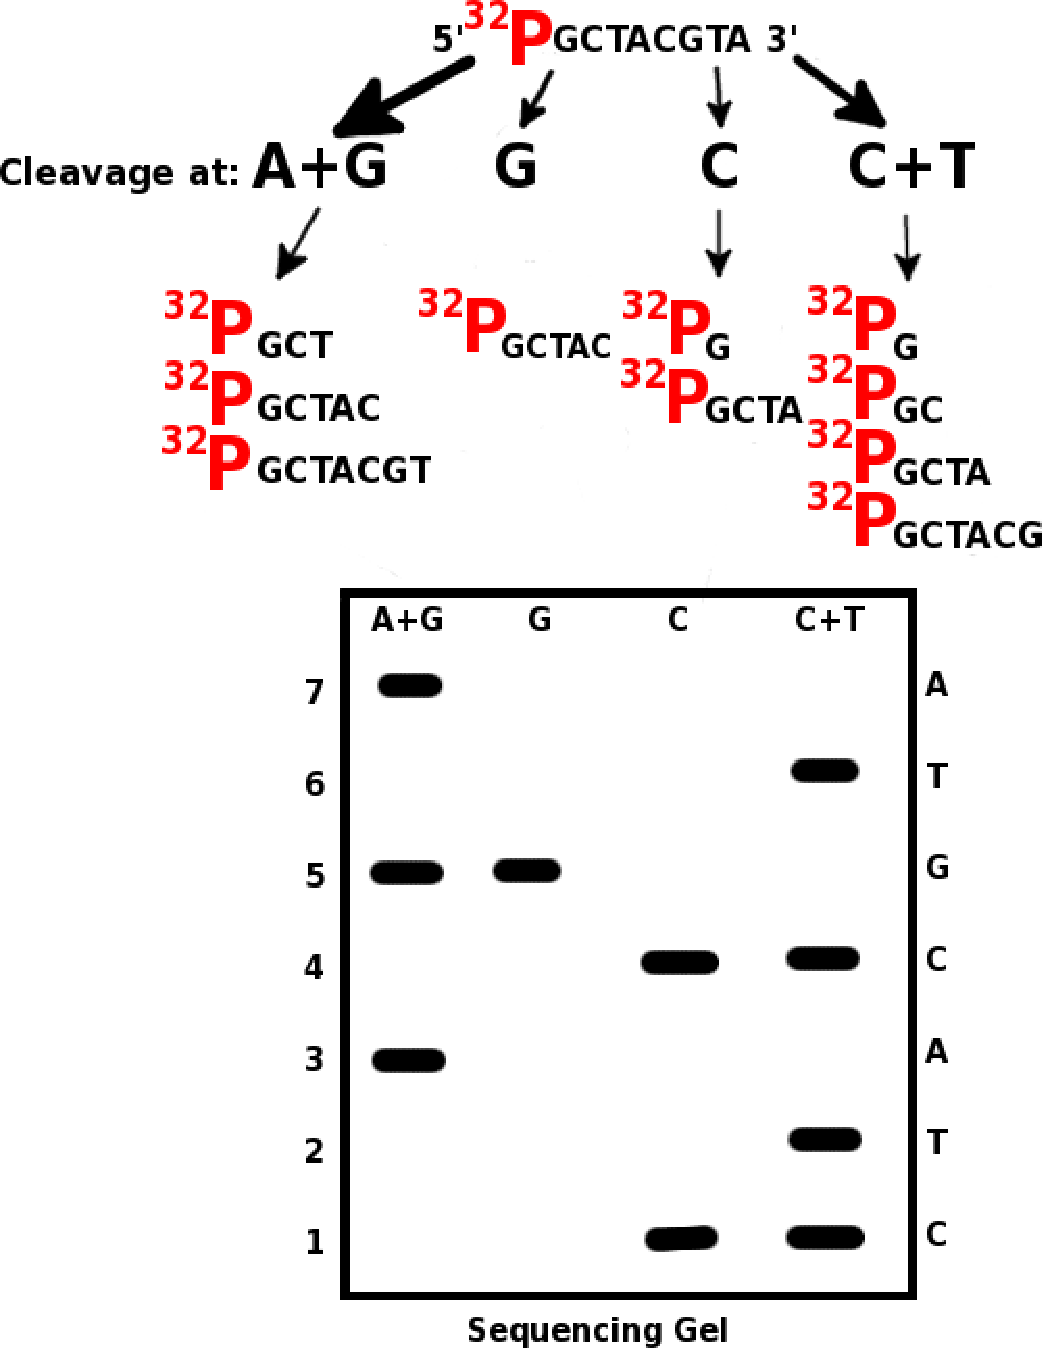
\includegraphics[width=.7\textwidth]{images/MG_2.pdf}
    \caption{}\label{fig:MGpro}
  \end{subfigure}%   
  \hfill
  \begin{subfigure}[b]{.5\linewidth}
    \centering
    \includegraphics[width=.99\textwidth]{images/MG_Chem.pdf}
    \caption{}\label{fig:MGchem}
  \end{subfigure}%    
  \caption{(a)   (b) }\label{fig:MG}
\end{figure}

When the method was developed Maxam \& Gilbert were able to get 100bp reads within a few days. 
By 1980, they had refined the technique to get 250bp reads and by 1995 the process had been 
automated by Dolan et al (1995) with 
500bp sequences. At the time when the method was developed this method was used because 
it did not rely on PCR
amplification and it could be easily controlled in the lab. However, the necessity of handling some 
pretty nasty chemicals
and the rather long wait times to produce sequence information made adopting new sequencing 
techniques attractive. 

\subsection*{Pyrosequencing}
Pyrosequencing is real time DNA sequencing (sequencing by synthesis) that detects the 
release of PPi as DNA polymerase forms
phosphodiester bonds between nucleotides. The technique was developed by  Mostafa Ronaghi 
and Pål Nyrén in XXXX. 
The really cleaver mechanism behind pyrosequencing is the use of the enzyme luciferase.
Luciferase is a general class of enzymes used in bioluminescence; the specific one used in 
pyrosequening
is that of fireflies \textit{P. pyralis}. The entire process is accomplished in three reactions: 

\begin{equation*}
\begin{aligned}
& (DNA)_n + dNTP \xrightarrow{DNA polymerase} (DNA)_{n+1} + PPi \\
& PPi + APS  \xrightarrow{ATP sulphurylase} ATP + SO_4^{-2}\\
& PPi + luciferin + O_2 \xrightarrow {luciferase} AMP + PPi + oxyluciferin + CO_2 + hv 
\end{aligned}
\end{equation*}


First DNA is exposed to one dioxyribonucleic acid at a time. If the nucleotide introduced is the
complementary base for the next position in the sequence DNA polymerase will encorporate it
creating a phosphodiester bond and releasing PPi. Another enzyme ATP sulphyrylase converts the
PPi and APS to ATP and $SO_4^{-2}$. This second reaction is needed to generate ATP that will be used
by the enzyme luciferase. In the final step the luciferin, a light-emitting compound,
and PPi react in the presence of oxygen to form AMP, PPi, oxyluciferin, carbon dioxide and light ($hv$).
After introducing a single nucleotide base, light emission indicates if the base was used by DNA 
polymerase. The amount of light produced indicates if more than one base is added in sequence. 

\begin{figure}[H]
\centering
    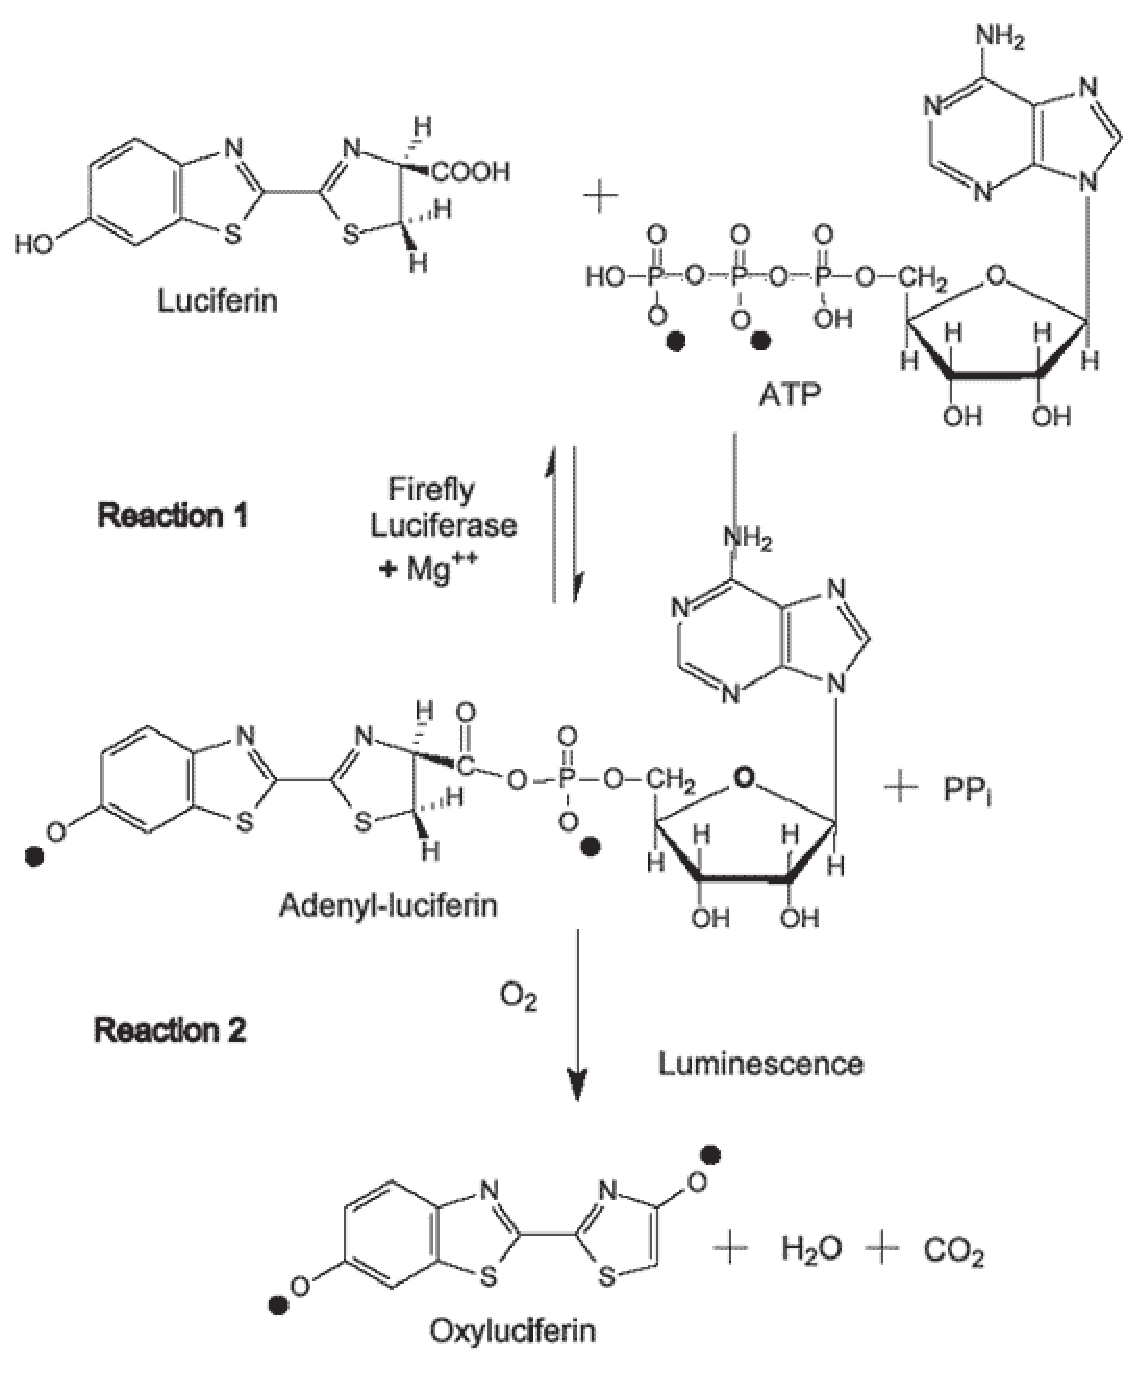
\includegraphics[width=.5\textwidth]{images/Luciferase.pdf}
    \caption{}\label{fig:Pyro} 
\end{figure}

Pyrosequencing can be divided into two general types: solid and liquid phase. Solid phase was described
by Ronaghi et al. in 1996. This method requires introducing a single nucleotide, washing the templete 
thouroughly before subsequent nucleotide additions to remove non-incorporated dNTPs and ATP. The
liquid phase method was describe by Ronaghi et al. in 1998. Instead of washing the templete between
dNTP introductions the nucleotides are degraded by the enzyme apyrase.
 
Pyrosequening has some pretty clear advantages over previous methods. The is no need for
labelled primers or nucleotides. Sequencing solely relies on the emission of light! There is also
no need for gel electrophoresis, so there is less dealing with acrylamide and other nasty chemicals.
Sequencing is done rapidly. Chain extension is accomplished in the 2min cycle time. All sequencing is
accomplished at room temperature and at physiological pH. Over the course of adopting this technology
some difficulties have been encountered. The solid phase method has issues with signal loss as the template
is washed repeatedly. Similarly, in the liquid phase method apyrase activity decreases over time such that
nucleotides and ATP are not completely digested before the next introduction. Despite its advantages  
pyrosequening is not a technique that many people will be adopting in the future. The GS FLX platform 
could read 400Mb in a 10 hour run, but each run cost between \$5,000 and \$7,000. 
Roache purchased the technology from Qiagen and promptly discontinued the entire line in 2013 and will
only be servicing these platforms through mid 2016. 

\subsection*{Massively parallel signature sequencing}
Massively parallel signature sequencing is a technique developed in the 1990s by Lynx therapeutics. It is a 
complicated bead based sequencing method that uses adapter ligation and decoding to sequence in chunks
of four nucleotides at a time. Because the process was so complex the method was never adopted by any
research labs other than Lynx. They predominantly used it for gene expression sequencing. Lynx merged with
Solexa, which was later aquired by Illumina, but the technology quickly became obsolete as much less complicated
approaches were designed. 

The general method is to attach anti-tags to microbeads, prepare cDNA with 5' flourcensent primers and 3' tags
by cloning them into a vector, load the beads with the labeled cDNA, sort the beads using flourecent-activated 
cell sorting (FACS), ligate an adapter to the cDNA, use probes to read four bases that are exposed to the adapter, 
then use an restriction enzyme to expose the next four bases for the next adapter. Generally you get ~17bp of
good sequence, but you also get a measure of the amount of mRNA in the cell. The microbeads are prepared
with a 3' spacer and the anti-tag. The sample mRNA is prepared by creating cDNA, labeling it with biotin so
that it sticks to the microbeads, inserting it into the vector creating tag-cDNA conjugate libraries, which were
then amplified using the flanking PCR primers. The amplified DNA was made single stranged and incubated 
with the anti-tag microbeads. The beads with the highest flourescence are sorted out and sequencing is started.
The sequencing process begins by cleaving the cDNA template using DpnII producing a 3-base overhang. 
The initiating adapter is ligated and 16 decoder probes are used to establish the identity and order of the 
nucleotides in the sequence four bases at a time. The adapter has a Bbv1 restriction site which 
codes for cleavage producing a 4bp overhang on the template sequence. This allows for the next adapter to ligate
and the process to sequence the next 4bp set. Typically this mehtod produced ~17bp of quality sequence information
and was used extensively in gene expression in house by Lynx. 

 \begin{figure}[H]
\centering
  \begin{subfigure}[b]{.5\linewidth}
    \centering
    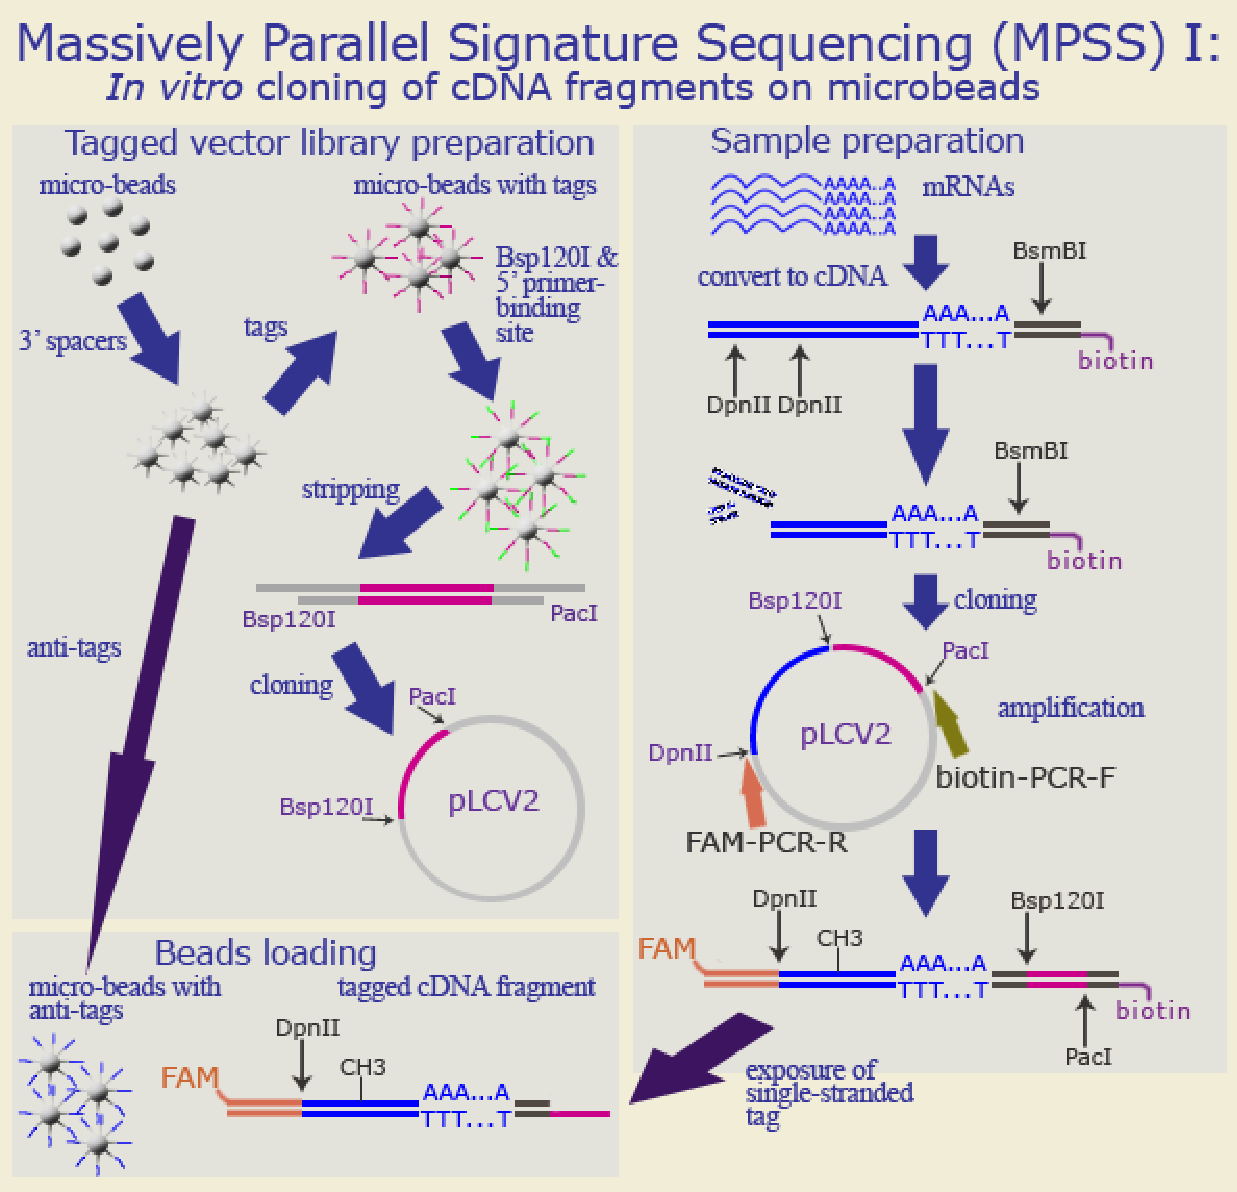
\includegraphics[width=.8\textwidth]{images/MPSS1.pdf}
  \end{subfigure}% 
  \begin{subfigure}[b]{.5\linewidth}
    \centering
    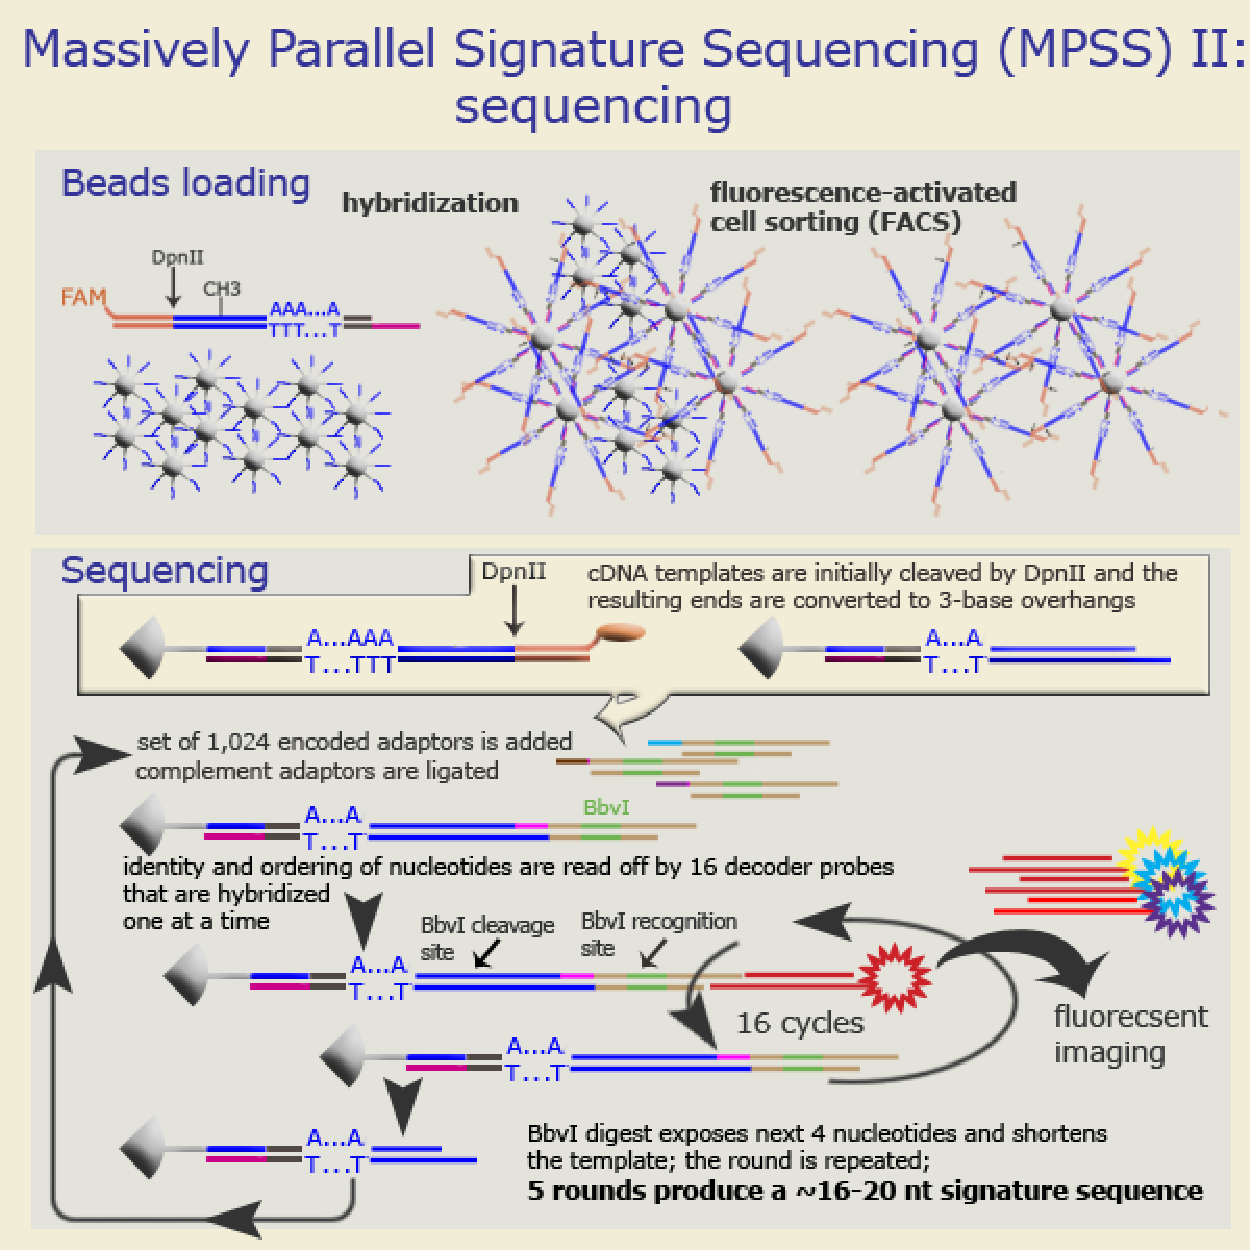
\includegraphics[width=.8\textwidth]{images/MPSS2.pdf}
  \end{subfigure}%    
  \caption{Massively parallel signature sequencing (MPSS) is a 
complicated bead based sequencing method that uses adapter ligation 
and decoding to sequence in chunks
of four nucleotides at a time. }\label{fig:MPSS}
\end{figure}

\subsection*{Polony Sequencing}
Developed by Church at Harvard in XXXX. This method uses in vitro paired-tag library with emulsion PCR, 
automated epifluorescence microscope and ligation based sequencing chemistry. It is open source, 
which is awesome! Polony sequencing is similar to MPSS in that it uses \textit{in vitro} cloning and hybridization
and ligation for sequencing. 
The first step of this method is preparing the paired end-tag library. Do do this genomic DNA is sheered.
Sheered DNA is then modified by the addition of an A to the 3' end and damaged is 
repaired by the converstion to 5' phosphorylated, blunt ended DNA. Gel electrophoresis is used to select for
fragements of 1Kb. Each of these fragments are cirularized using a T-tailed 30bp long synthetic 
oligonucleotide (T30) which has two MmeI recognition sites that cut within the template strand sequence.
Rolling circle amplification increases the number of amplicon and MmeI is used to cut our the T30 sequence
flanked by ~17-18bp of the sequence. Emulsion PCR (ePCR) primers, specificcally FDV2 and RDV2, are
ligated onto the fragment and PCR is used to obtain a library of 135bp fragments (FDV2 primer - sequence - 
T30 - sequence - RDV2 primer). This fragment is then amplified many times over on the surface of a streptavidin
coated bead. The beads are preloaded with biotin labeled forward primer. The beads, PCR mixture, paired end-tag
library are all mixed to create an emulsion. Theoretically one drop of water in the oil emulsion has one bead
and one molecule of DNA attached. PCR is performed to produce either beads with zero (if no DNA molecule is 
bound to the bead), clonal (if 1 DNA molecule is bound to the bead), or non-clonal (if multiple DNA molecules are 
bound to the bead). After PCR, the emulsion is broken with detergent and isopropanol. Beads are then enriched 
by using plystyrene beads that have been preloaded with biotinylated capture oligonucleotides. These beads 
bind to beads that have amplified DNA. Beads lacking amplified DNA can be separated out with centrifugation.
An amino cap is added to the 3’ end of both unextended forward ePCR primers and the RDV segment of template DNA. 
A coverslip is washed and treated with aminosilane to allow covalent coupling of DNA. The amplified enriched beads are 
then mixed with acrylamide and poured inot a shallow mold framed by a teflon coated microscope slide. The coverslip
is placed over the bead/acrylamide mix and allowed to polymerize after which the slide is removed. DNA sequencing
is accomplished by introducing anchor primers through the cell and allowing them to hybridize with the 3' or 5' end of 
the genomic DNA tags. The anchor primers are then ligated to fluorescently labelled degenerate nonomers. 
These nonamers are 9 bases long and are differentially
labeled allowing the identification of which base is located in the query position specific to the nonamer. 
The fixation of the fluorescent molecule signals the identity of the base. 
The primer and nonomer complex is then stripped off and a new primer is replaced so that the next fluorescently 
labeled nonomer with the query position shifted one base can be ligated. 

\begin{figure}[H]
\centering
    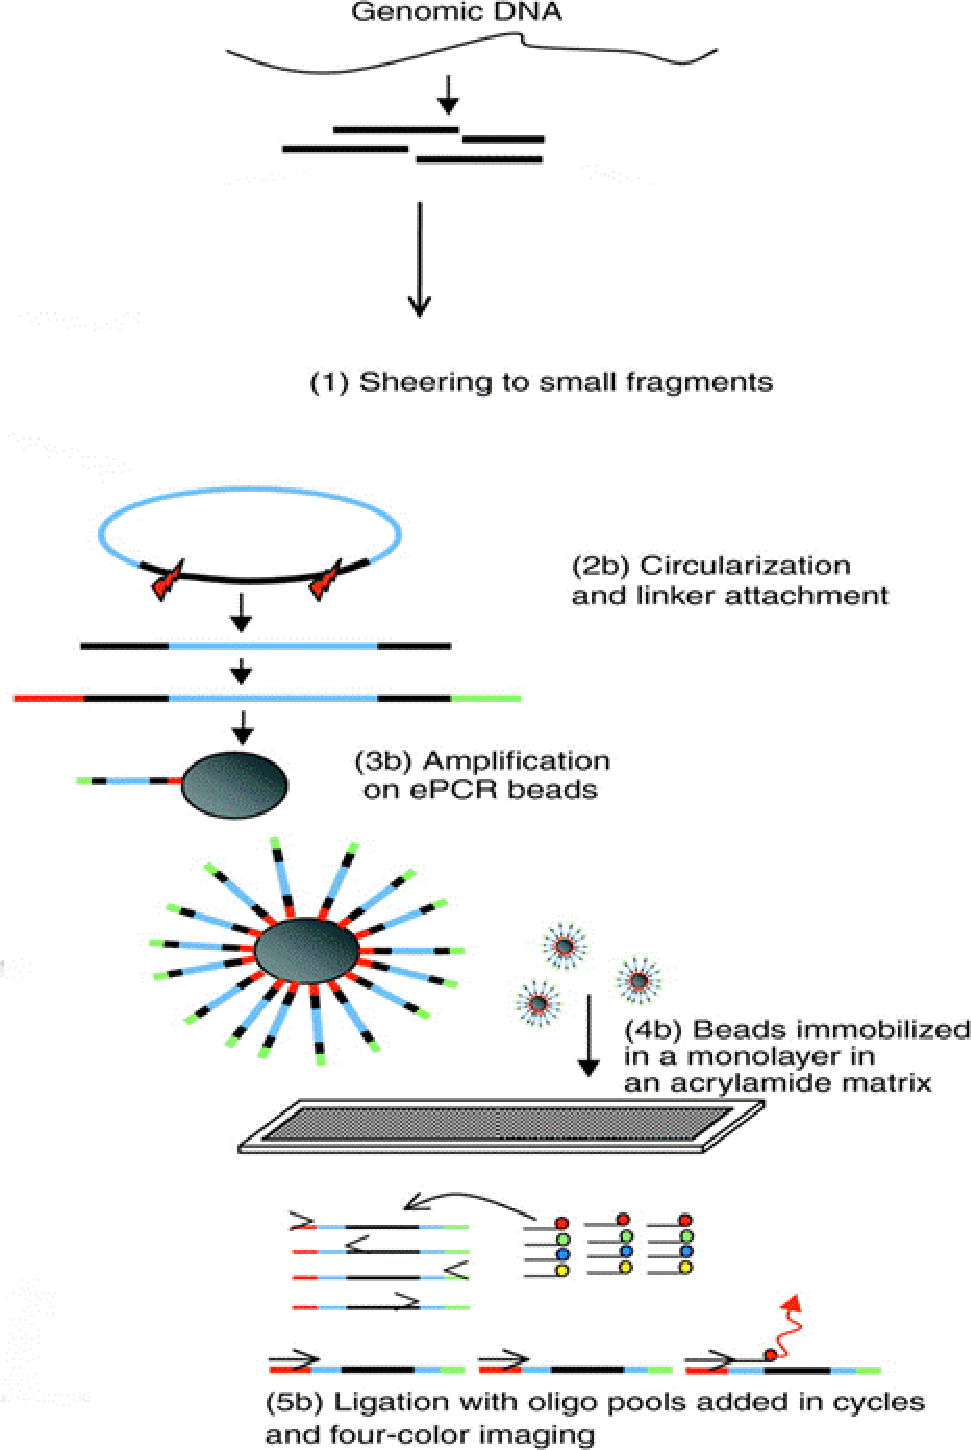
\includegraphics[width=.3\textwidth]{images/Polony.pdf}
    \caption{}\label{fig:Polony} 
\end{figure}

This process produces millions of ~26bp reads (13bp on either end), however, only about 1 bit 
for every 10,000 bits collected is useful. The technology was licensed to Agencourt Biosciences, later 
picked up by Applied Biosystems. The methodology forms the basis for the ABI solid sequencing method.

\subsection*{Illumina (Solexa) sequencing}
Solexa founded by Shankar Balasubramanian and David Klenerman in 1998 developed a sequencing technique
that uses colony amplification of DNA fragments on a flowcell combined with reversible terminator nucleotides 
for massively parallel sequencing by synthesis. Solexa merged with Lynx and was later aquired by Illumina. 

The basic method consists of attaching DNA to the surface of a flowcell, bridge amplification, and sequencing 
by synthesis. The DNA is first fragmented and adapters are ligated to both ends. The DNA is then made single 
stranded and bound to the surface of a flow cell channel. The flow cell is made of up 8 lanes, each of which 
has 3 columns with 100 tiles per column. has dense lawns of primers. Bridge amplification
is accomplished by introducing unlabelled nucleotides nad enxymes. The dense lawns of primers use the newly 
attached fragments as a templete making dsDNA. The dsDNA is denatured and the cycle is repeated yieldign dense
clonal colonies. Sequencing is then done on the flowcell that has dense clonal colonies. Similar to Sanger sequencing, 
this method of sequencing takes advantage of being able to add a special nucleotide that inhibits the addition of another
base by blocking addition at the 3'OH. Instead of using ddNTP that that effectivly block all further addition of bases
this method uses reversible terminator nucleotides that when added block the addition of another nucleotide until
an image has been take of the fluorescence of the colony indicating the last base added after which 
enzymatic cleavage removes the 3'OH block and fluorecent dye allowing the incorporation of the next nucleotide.  

\begin{figure}[H]
\centering
    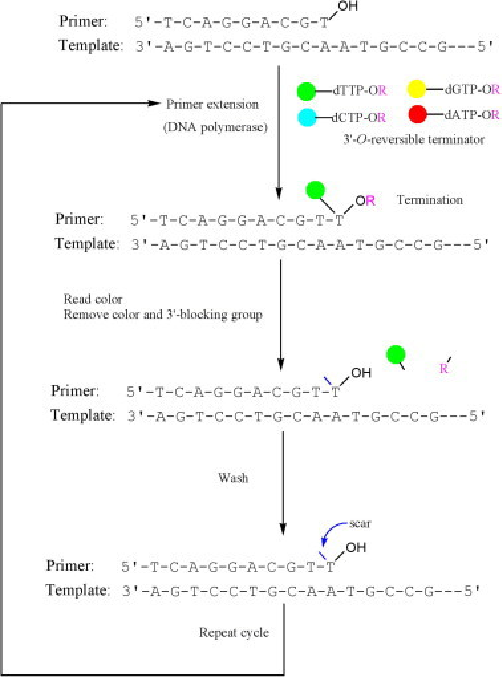
\includegraphics[width=.3\textwidth]{images/Solexa.pdf}
    \caption{}\label{fig:Solexa} 
\end{figure}

Solexa allows the rapid accumulation of sequence data. You end up with ~40 million reads per run and 
1 billion base pair per run. All four nucleotides being present during sequencing minimizes
incorporation bias. 
There are a few downsides to Solexa sequencing. Reads are on average 36bp. While reads 100bp in length
are often cited, error rates at 36bp are about 2\%. With such small reads, de novo assembly is impossible, so without 
a reference genome for alignment you're SOL.  

\subsection*{SOLiD sequencing}
SOLiD sequenicng uses the same basic method as Polony sequencing - sequencing by ligation. DNA libraries are first
contructued by fragmenting the DNA and then adding adapters. DNA is attached to beads and ePCR is used to 
increase the copy number on each bead. The beads are attached to a glass slide and then sequencing is done via 
probes that compete for ligation. The main differences specific to the SOLiD platform are the use of P1 adapters 
for the known primer sequence and the specifics behind the ligation step. 
While Polony sequencing used nonomers that identified 1 base, the SOLiD platform makes use of 
fluorecently labelled di-base probes so that two bases can be infered at a time. The di-base probe
is specific to the first and second position for each ligation reaction. After ligation of a probe an image is taken
and the fluorecent dye is cleaved off and the next probe and anneal and ligate to reveal two more bases in the
sequence. Multiple cycles of ligation, flourescent detection and cleaveage are done and then the extension product
is removed and a new primer complementary to the n-1 position anneals and the next set of ligation cycles are
performed. In total five rounds of primer reset are completed. 

 \begin{figure}[H]
\centering
  \begin{subfigure}[b]{.5\linewidth}
    \centering
    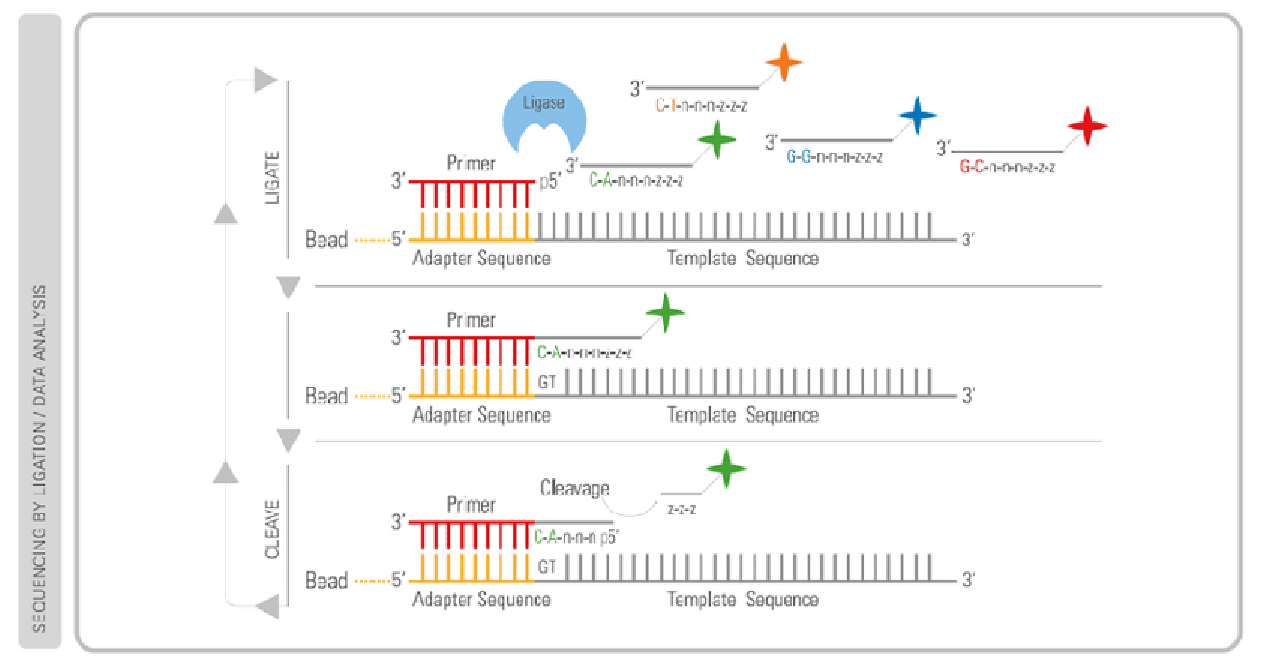
\includegraphics[width=.8\textwidth]{images/SOLiD1.pdf}
  \end{subfigure}% 
  \begin{subfigure}[b]{.5\linewidth}
    \centering
    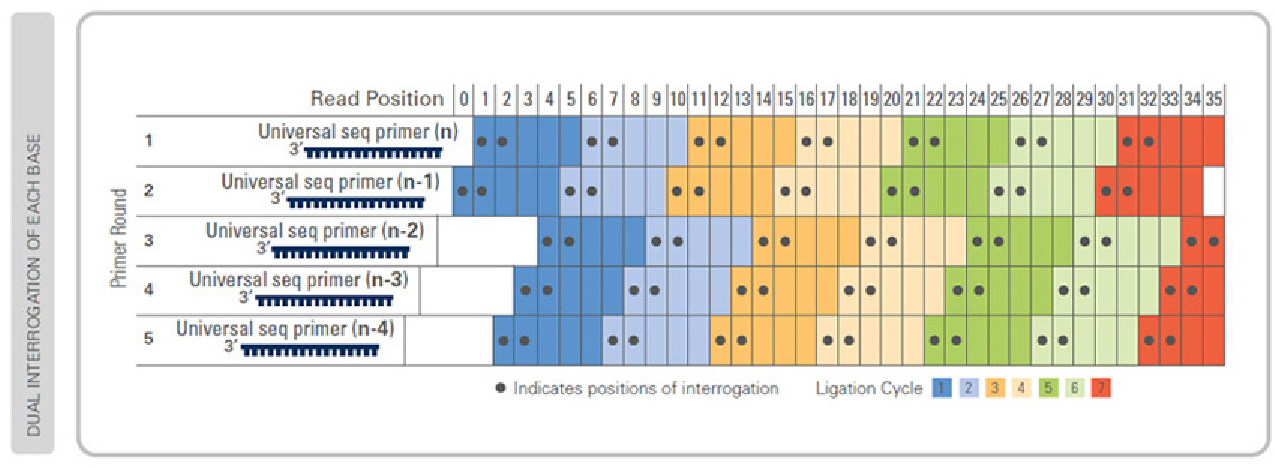
\includegraphics[width=.8\textwidth]{images/SOLiD2.pdf}
  \end{subfigure}%    
  \caption{ }\label{fig:SOLiD}
\end{figure}

Having a di-base probe means that each query position of the probe is assessed in two rounds of primer reset making
this type of assay very accurate. Some issues with palindromic seqeunces have been noted (Yu-Feng Huang et al. 2012). 

Applications: Sequencing of course. Transcriptome for non-model organisms. Microarrays are limited to what is on the chip, which is 
not the case for sequencing. Expression profiling is possible as quantitative reads have been done!

\subsection*{Ion Torrent semiconductor sequencing}
There is nothing really all that novel about the chemistry behind how the sequencing is accomplished, 
what is novel is the detection method. The Ion Torrent is able to detect hydrogen ions that are 
released as DNA polymerization occurs. Similar to pyrosequencing that detects the release of light, 
the special semiconductor is hypersensative to hydrogen ions (ISFET). First a DNA library is constructed by 
fragmenting DNA and adding adapters. Fragmented DNA is then placed on a microbead and amplified.
 Each bead then occupies a microwell that is 
flooded with a single type of nucleotide at a time. If the nucleotide is encorporated by DNA polymerase
hydrogen ions will be released and detected. If there is a run of a single nucleotide, many ions will 
be released and a larger signal will be detected. 

Relatively cheap and really fast! A typical run takes about an hour and sequence lengths are typically 
100-200bp long. Long runs of a single nucleotide are difficult to enumerate (this problem is shared with 
pyrosequencing). 

\subsection*{DNA nanoball}
In 2006, Clifford Reid, Radoje Drmanac, and John Curson came together to found Complete Genomics 
and a proprietary way of sequencing. What is interestesting about these guys is that they do not sell 
their platform, the company sequences samples sent in by reserachers. Their cost is \$20,000 per genome,
with a minimum of eight genomes. 

DNA is sheered into ~500bp fragments. Then adapters are ligated onto the ends of each fragment. These
adapters have restriction enzyme recognition sites that are inside the template DNA. Three more 
rounds of adapter ligation and circularization are performed so that the end product is a circular fragment of 
DNA that is composed of the first adapter Ad1, a 13bp fragment of genomic DNA, the second adapter Ad2, a 26bp 
genomic fragment, 
the forth adapter Ad4, a second 26bp genomic fragment, the third adapter Ad3, and a 13bp genomic 
fragment of DNA. 

The circular DNA is then amplified by rolling circle amplification using 
Phi 29 DNA polymerase. This produces long single stranded DNA and the adapter 
sequences have palindromic sequences that interact to make the DNA curl up into
a tight ball ~300 nanometers in diameter. The DNA nanoballs are then attached
to the surface of a flowcell. The flowcell is silicone chip with 'sticky spots' where 
one nanoball can attach. Sequencing of genomic DNA between adapters is accomplished
with the ligation of fluorescently labelled probes. Anchor sequences are introduced to 
bind to the adapter sequence. T4 DNA ligase and a pool of 4 10-mer DNA probes with 
degenerate nucleotides on all but 1 position (the query position) are introduced. If the probe
has a complementary sequence it will bind to the template DNA and the ligase will add the 
probe to the anchor sequence. The unincorporated probes are washed away and an image
is taken using the fluorescent dye attached to the probe to indicate which base is in the 
query position. The anchor/probe complex is removed and a new anchor and pool of 
probes this time with the query position located one base downstream. After all 10 positions
of the probe are infered, a new anchor that binds to a different adapter is introduced and 
the next genomic fragment is sequenced. 

\begin{figure}[H]
\centering
    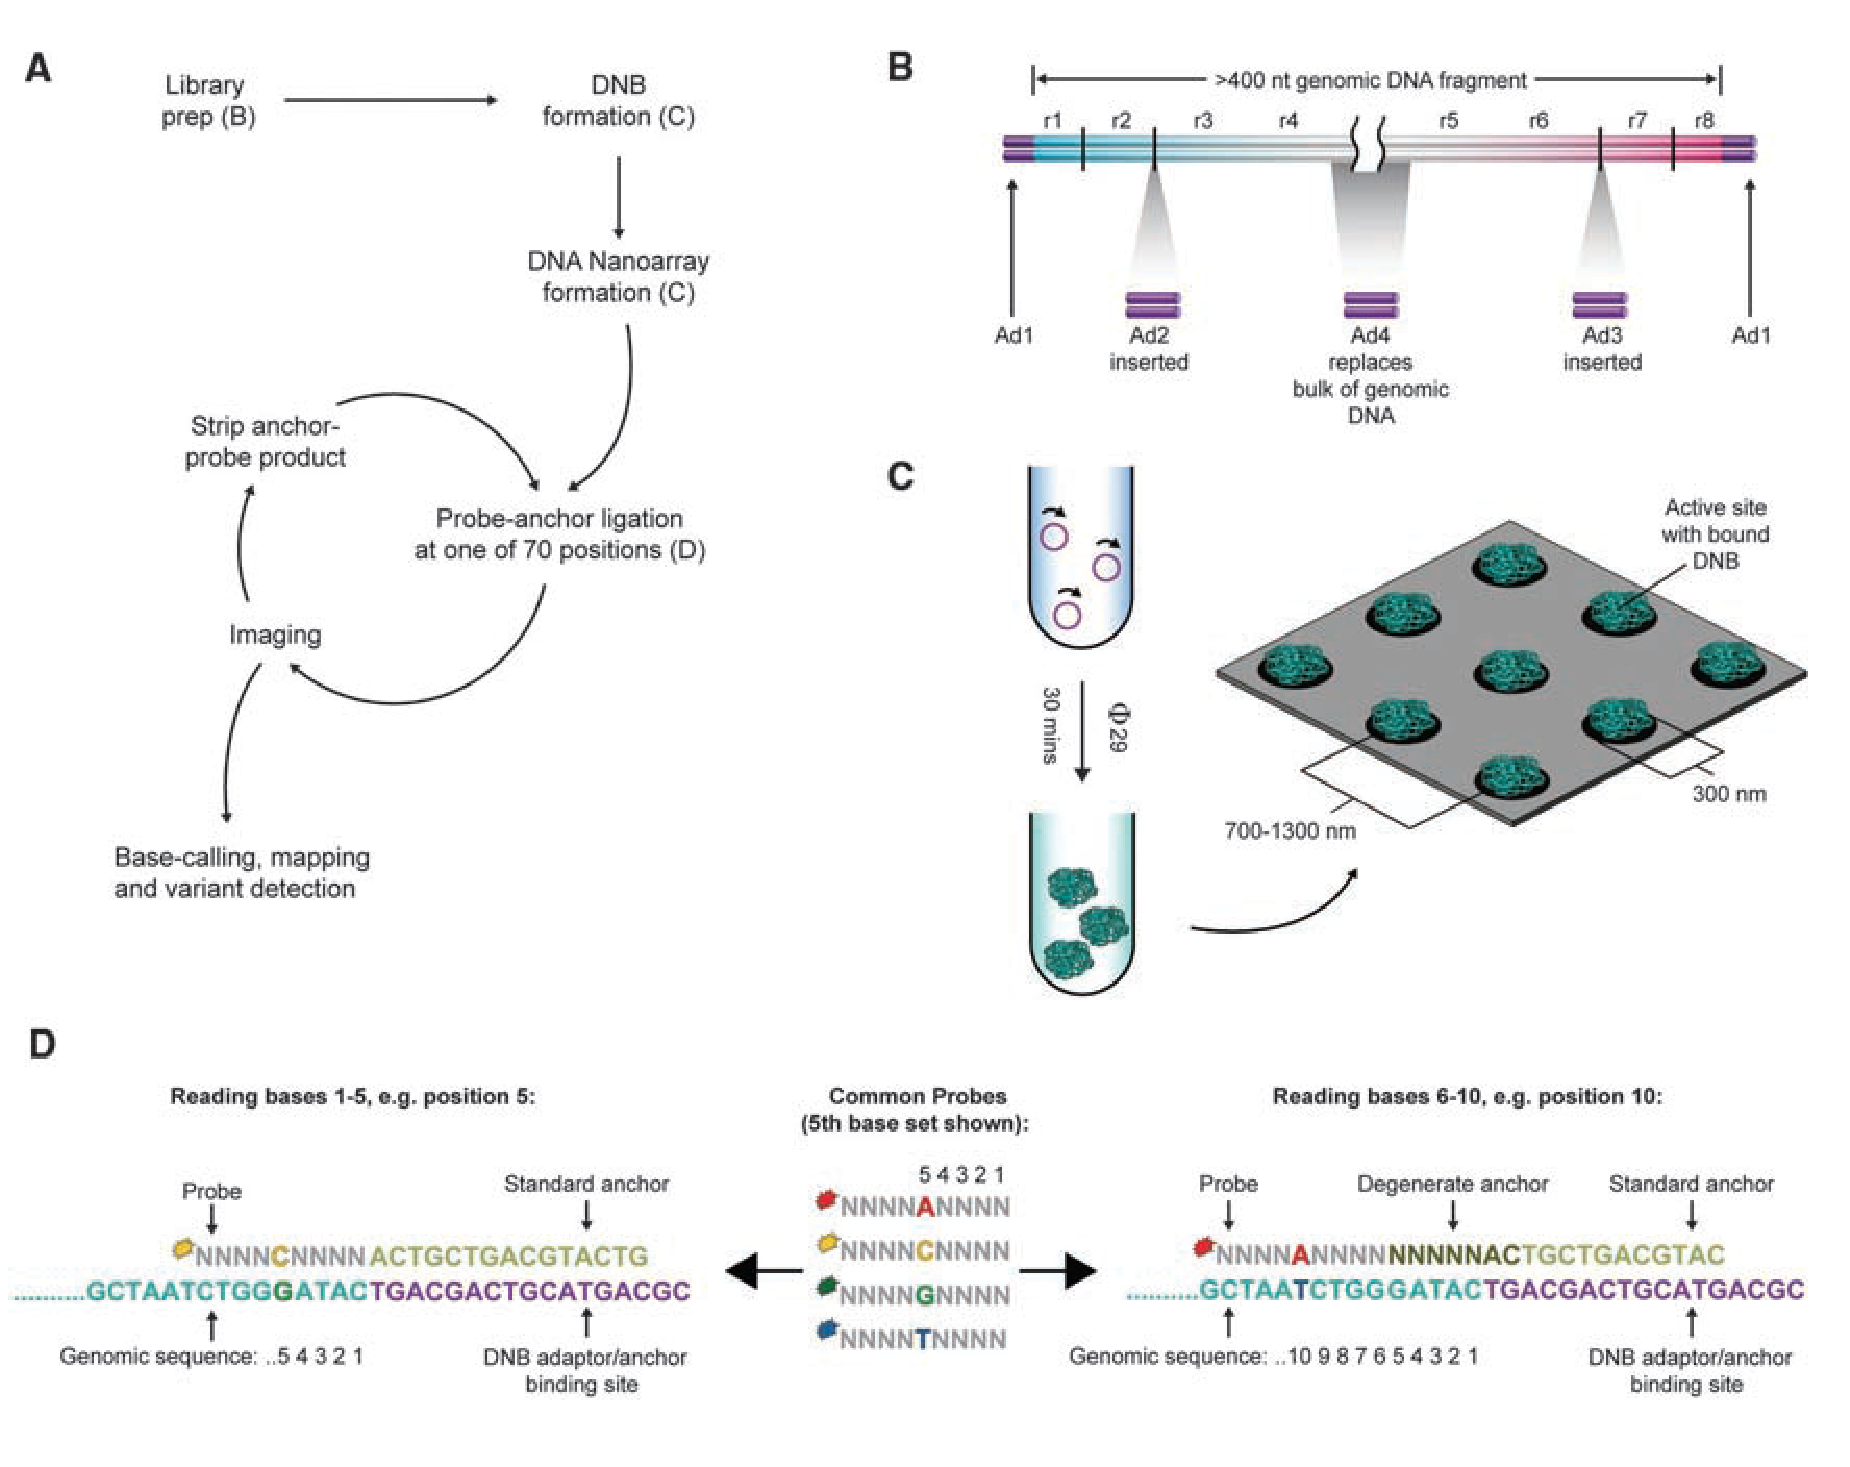
\includegraphics[width=.5\textwidth]{images/Nanoball2.pdf}
    \caption{}\label{fig:Nanoball} 
\end{figure}

One advantage to the nanoball method is the high density of the nanoballs on the flowcell.
Other methods typically have random placement on the flowcell, whereas one nanoball occupies
one 'sticky spot' on the nanoball array. Also, by using non-chained ligation the compentency 
of ligations deep in the read are not dependent on earlier ligations. 

The read length are pretty short. This makes the use of a reference genome critical 
for most applications. Many rounds of PCR amplification also mean that there is 
increased risk of contamination and errors associated with polymerization.

\subsection*{Heliscope single molecule sequencing}
Heliscope sequencing was developed by XXXX. 
The basic workflow is preparing the DNA library, attaching the library molecules to 
a flowcell, and then sequencing by synthesis. High molecular weight DNA is first 
sheered to obtain fragments to work with. Heliscope recommends fragments between 100 \&
200nt. A poly(dA) tail is next added to the DNA fragments that will bind to complementary 
sequences on the flowcell. Generating the exact same number of dAs and dTs is extremely difficult
and in order to only sequence the template it is easier to do some modifications to the 
anchor sequence on the flowcell before sequencing. Similarly, in order to keep the templete strand from 
polymerizing and adding
to its 3' end it must be blocked by adding a dideoxynucleotide with terminal transferase to 
its 3' hydroxyl end. The commerically available flowcell is prepared with an oligo(dT) sequence that is 50nt 
long. DNA is exposed to the flowcell and the poly(dA) tail should bind to the oligo(dT) sequence
on the surface of the flowcell. A 'fill \& lock' step is performed prior to sequencing where unpaired
dAs on the poly(A) tail are paried and Virtual Terminator nucleotides dATP, dCTP, dGTP are added
to fill in the template until an non-A is present halting elongation. Taking an image at this time
provides no information on the base identity, only the position of each DNA molecule 
capable of sequencing. The fluorescent dye and 3' block on the sequencing strand is then cleaved 
and the sequencing cycles can progress. During each cycle of the sequencing reaction 
a single fluorescent nucleotide is added, unincorporated bases are washed away, and an image 
is taken. Right now the rate limiting step is the image capturing step. 

\begin{figure}[H]
\centering
    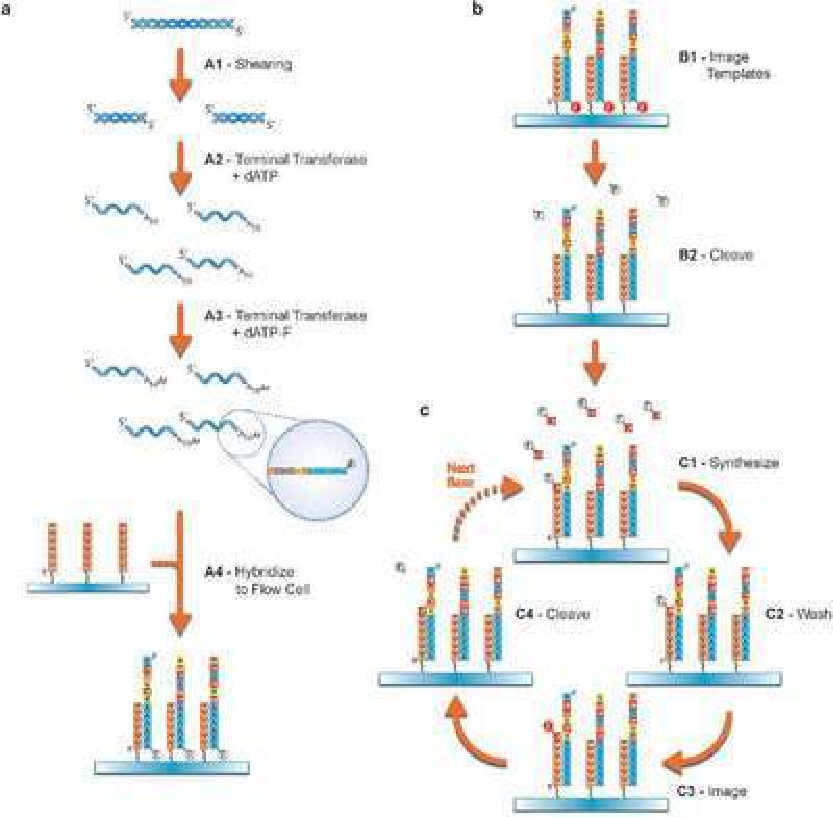
\includegraphics[width=.4\textwidth]{images/Helicos.pdf}
    \caption{}\label{fig:Nanoball} 
\end{figure}

One advantage of this process is the lack of PCR amplification that may introduce bias and
errors. The addition of single nucleotides at a time requires 4 images per base position leading 
to long processing times. Similarly, read lengths are typically 32 nt long. 


\subsection*{Single molecule real time sequencing}
Single molecule real time (SMRT) sequening was developed by Eid et al. at PAcific Biosciences. 
It uses a special nanostructure, a zero mode wave-guide (ZMW), that houses a single 
DNA polymerase enzyme and single DNA molecule at the bottom of a small well (Fig \ref{fig:SMRT}). 
The ZMW structure allows the illumination of fluroescent dyes that are being incorporated into the 
growing DNA chain individually. The fluroescent dye is linked to the phosphate chain such
that when the phosphodiester bond is formed the dye is cleaved and diffusion carries the 
fluorescent dye away from the detection area of the chamber. The ZMW chamber 
is located on a 93x33 well chip. The result is massively parallel real time sequencing of 
a single molecule of DNA. 

\begin{figure}[H]
\centering
    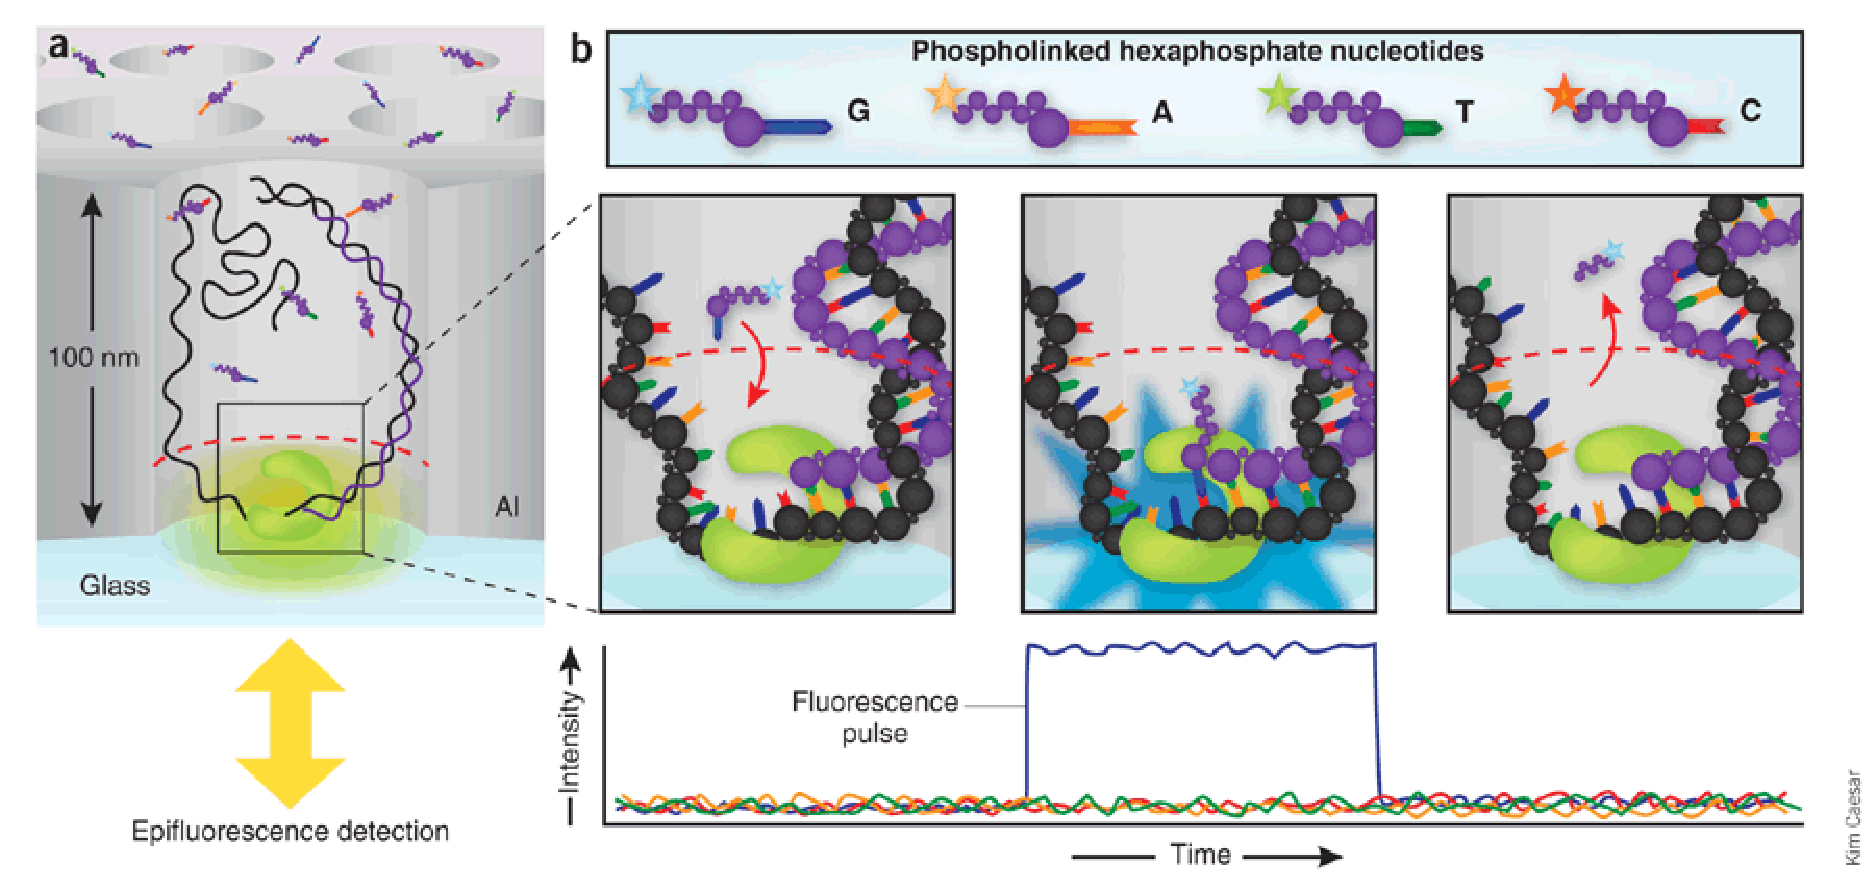
\includegraphics[width=.8\textwidth]{images/SMRT.pdf}
    \caption{}\label{fig:SMRT} 
\end{figure}

Researchers have achieved reads between 1.1 \& 7Kb in length. 
As the chemistry is refined reads have
progressively lengthened. This is a major advantage as it offers an opportunity for 
\textit{de novo} genome assembly. Similarly the polymerization chemistry allows for
methylation detection. The method is not without problems. 
Only about 1/3 of the ZMWs can be populated with a single DNA polymerase. 
Similarly, high error rates have been reported for single reads. However,
when 15 or more reads are done accuracy is $>$99\%. 

\section{Single Nucleotide Polymorphisms (SNPs)}
Who developed it, how it was done, pros cons

\subsection{Genotyping by sequencing}




\chapter{Population Genetics}
\section{Hardy-Weinberg Principle}
\section{Mutation}
\section{Drift}
\section{migration}
\section{Selection}


\end{document}  
